\documentclass[18pt,xcolor=table]{beamer}

%!TEX root = ./main.tex
\usepackage {bbm}
\usepackage {textpos}
\usepackage {tikz}
\usepackage {graphicx}


\definecolor{blue1}{RGB}{176,196,222 }
\definecolor{blue2}{RGB}{54,100,139}

\definecolor{grey1}{RGB}{139,139,131}
\definecolor{grey2}{RGB}{235,235,235}

\definecolor{black1}{RGB}{50,50,50}

\mode<presentation>
{
  % \usetheme{Pittsburgh}   
  %\usetheme{Boadilla}  
\usetheme{Madrid}  
  \usefonttheme[onlymath]{serif}
  \setbeamertemplate{items}[circle] 
  \setbeamertemplate{sections/subsections in toc}[circle]
  \setbeamercovered{invisible}
  \setbeamertemplate{navigation symbols}{}
% \usecolortheme{seahorse}
%
%  % Color Theme 
  \setbeamercolor{normal text}{bg=white,fg=black1} %All standard text
  \setbeamercolor{structure}{fg=blue2} %% Table of Contents 

  \setbeamercolor*{frametitle}{fg=black1,bg=grey2} % Frame title colors
%  \setbeamerfont{frametitle}{series=\bfseries}
  \setbeamercolor*{framesubtitle}{fg=blue2} % Frame subtitle color

  \setbeamercolor*{palette primary}{use=structure,fg=black1, bg=grey2} %right bottom
  \setbeamercolor*{palette secondary}{use=structure,bg=blue1} %middle bottom
  \setbeamercolor*{palette tertiary}{use=structure,bg=blue2,fg=grey2} %left bottom

  \setbeamercolor*{block body}{fg=black1,bg=blue1!10} % Color of blocks
  \setbeamercolor*{block title}{parent=structure,fg=black1,bg=blue1} % Block Titles
  \setbeamercolor{alerted text}{fg=blue2!85!black,} % Alerted Text (ie. highlight with \alert)
  \setbeamerfont{alerted text}{series=\bfseries}

  % not sure what these do.
  \setbeamercolor{item projected}{use=item,fg=black1,bg=item.fg!35}
  \setbeamercolor*{block title alerted}{parent=alerted text,bg=black1!15}
  \setbeamercolor*{block title example}{parent=example text,bg=black1!15}
  \setbeamerfont{framesubtitle}{size=\small}
}

\makeatletter
\setbeamertemplate{footline}
{
  \leavevmode%
    \hbox{%
      \begin{beamercolorbox}[wd=.333333\paperwidth,ht=2.25ex,dp=1ex,center]{author in head/foot}%
        \usebeamerfont{author in head/foot}\insertshortauthor%~~\beamer@ifempty{\insertshortinstitute}{}{(\insertshortinstitute)}
      \end{beamercolorbox}%
        \begin{beamercolorbox}[wd=.333333\paperwidth,ht=2.25ex,dp=1ex,center]{title in head/foot}%
        \usebeamerfont{title in head/foot}\insertshorttitle
        \end{beamercolorbox}%
        \begin{beamercolorbox}[wd=.333333\paperwidth,ht=2.25ex,dp=1ex,right]{date in head/foot}%
        \usebeamerfont{date in head/foot}\insertshortdate{}\hspace*{2em}
        \insertframenumber{} / \inserttotalframenumber\hspace*{2ex} 
      \end{beamercolorbox}}%
        \vskip0pt%
}
\makeatother

%\usepackage{kerkis}
\usepackage{helvet} 
\usepackage[T1]{fontenc}
\usepackage[protrusion=true,expansion=true]{microtype}
\usepackage{amsmath}

\renewcommand*{\thefootnote}{\fnsymbol{footnote}}


\pgfdeclareimage[height=1.5cm]{logo}{./logos/hd_logo}
\pgfdeclareimage[height=0.8cm]{small_logo}{./logos/hd_logo}

\AtBeginSection[] { 
  \begin{frame}[plain] 
    \frametitle{\bf Outline:}
    \framesubtitle{~~} 
    \tableofcontents[currentsection] 
  \end{frame} 
  \addtocounter{framenumber}{-1} 
} 

\setbeamercovered{transparent}

%%%%%%%%%%%%%%%%%%%%%%%
% user-defined commands
%%%%%%%%%%%%%%%%%%%%%%%
%!TEX root = ../main.tex


\newcommand{\beq}{\begin{equation}}
\newcommand{\eeq}{\end{equation}}

\newcommand{\eq}[1]{\begin{align*}#1\end{align*}}

\newcommand{\bfi}{\begin{figure}}
\newcommand{\efi}{\end{figure}}

\newcommand{\icg}{\includegraphics}

\newcommand{\bdm}{\begin{displaymath}}
\newcommand{\edm}{\end{displaymath}}

\newcommand{\beqa}{\begin{eqnarray}}
\newcommand{\eeqa}{\end{eqnarray}}

\newcommand{\beqas}{\begin{eqnarray*}}
\newcommand{\eeqas}{\end{eqnarray*}}

\newcommand{\barr}{\begin{array}}
\newcommand{\earr}{\end{array}}

\newcommand{\bit}{\begin{itemize}}
\newcommand{\eit}{\end{itemize}}

\newcommand{\qq}[1]{\qquad \mbox{#1} \qquad}

\def\hyph{-\penalty0\hskip0pt\relax}

% Tikz
\definecolor{blue1}{RGB}{176,196,222 }
\definecolor{blue2}{RGB}{54,100,139}
\definecolor{grey1}{RGB}{139,139,131}
\definecolor{grey2}{RGB}{235,235,235}
\definecolor{black1}{RGB}{50,50,50}


%Spaces
\newcommand{\Sp}[1]{{\cal #1}}
%
\newcommand{\sA}{\Sp{A}}
\newcommand{\sB}{\Sp{B}}
\newcommand{\sC}{\Sp{C}}
\newcommand{\sD}{\Sp{D}}
\newcommand{\sE}{\Sp{E}}
\newcommand{\sF}{\Sp{F}}
\newcommand{\sG}{\Sp{G}}
\newcommand{\sH}{\Sp{H}}
\newcommand{\sI}{\Sp{I}}
\newcommand{\sJ}{\Sp{J}}
\newcommand{\sK}{\Sp{K}}
\newcommand{\sL}{\Sp{L}}
\newcommand{\sM}{\Sp{M}}
\newcommand{\sN}{\Sp{N}}
\newcommand{\sO}{\Sp{O}}
\newcommand{\sP}{\Sp{P}}
\newcommand{\sQ}{\Sp{Q}}
\newcommand{\sR}{\Sp{R}}
\newcommand{\sS}{\Sp{S}}
\newcommand{\sT}{\Sp{T}}
\newcommand{\sU}{\Sp{U}}
\newcommand{\sV}{\Sp{V}}
\newcommand{\sW}{\Sp{W}}
\newcommand{\sX}{\Sp{X}}
\newcommand{\sY}{\Sp{Y}}
\newcommand{\sZ}{\Sp{Z}}

%Vectors
\newcommand{\V}[1]{{\bf #1}}
%
\newcommand{\va}{\V{a}}
\newcommand{\vb}{\V{b}}
\newcommand{\vc}{\V{c}}
\newcommand{\vd}{\V{d}}
\newcommand{\ve}{\V{e}}
\newcommand{\vf}{\V{f}}
\newcommand{\vg}{\V{g}}
\newcommand{\vh}{\V{h}}
\newcommand{\vi}{\V{i}}
\newcommand{\vj}{\V{j}}
\newcommand{\vk}{\V{k}}
\newcommand{\vl}{\V{l}}
\newcommand{\vm}{\V{m}}
\newcommand{\vn}{\V{n}}
\newcommand{\vo}{\V{o}}
\newcommand{\vp}{\V{p}}
\newcommand{\vq}{\V{q}}
\newcommand{\vr}{\V{r}}
\newcommand{\vs}{\V{s}}
\newcommand{\vt}{\V{t}}
\newcommand{\vu}{\V{u}}
\newcommand{\vv}{\V{v}}
\newcommand{\vw}{\V{w}}
\newcommand{\vx}{\V{x}}
\newcommand{\vy}{\V{y}}
\newcommand{\vz}{\V{z}}

\newcommand{\vA}{\V{A}}
\newcommand{\vB}{\V{B}}
\newcommand{\vC}{\V{C}}
\newcommand{\vD}{\V{D}}
\newcommand{\vE}{\V{E}}
\newcommand{\vF}{\V{F}}
\newcommand{\vG}{\V{G}}
\newcommand{\vH}{\V{H}}
\newcommand{\vI}{\V{I}}
\newcommand{\vJ}{\V{J}}
\newcommand{\vK}{\V{K}}
\newcommand{\vL}{\V{L}}
\newcommand{\vM}{\V{M}}
\newcommand{\vN}{\V{N}}
\newcommand{\vO}{\V{O}}
\newcommand{\vP}{\V{P}}
\newcommand{\vQ}{\V{Q}}
\newcommand{\vR}{\V{R}}
\newcommand{\vS}{\V{S}}
\newcommand{\vT}{\V{T}}
\newcommand{\vU}{\V{U}}
\newcommand{\vV}{\V{V}}
\newcommand{\vW}{\V{W}}
\newcommand{\vX}{\V{X}}
\newcommand{\vY}{\V{Y}}
\newcommand{\vZ}{\V{Z}}

\newcommand{\vone}{\V{1}}
\newcommand{\vzero}{\V{0}}
\newcommand{\B}{\V{B}}
\newcommand{\E}{\V{E}}
\newcommand{\Er}{\V{E}_r}
\newcommand{\Es}{\V{E}_s}
\newcommand{\un}{\hat{\vn}}



%Vectors
\newcommand{\T}[1]{\underline{\bf #1}}
%
\newcommand{\ta}{\T{a}}
\newcommand{\tb}{\T{b}}
\newcommand{\tc}{\T{c}}
%\newcommand{\td}{\T{d}}
\newcommand{\te}{\T{e}}
\newcommand{\tf}{\T{f}}
\newcommand{\tg}{\T{g}}
%\newcommand{\th}{\T{h}}
\newcommand{\ti}{\T{i}}
\newcommand{\tj}{\T{j}}
\newcommand{\tk}{\T{k}}
\newcommand{\tl}{\T{l}}
\newcommand{\tm}{\T{m}}
\newcommand{\tn}{\T{n}}
%\newcommand{\to}{\T{o}}
\newcommand{\tp}{\T{p}}
\newcommand{\tq}{\T{q}}
\newcommand{\tr}{\T{r}}
\newcommand{\ts}{\T{s}}
%\newcommand{\tt}{\T{t}}
\newcommand{\tu}{\T{u}}
\newcommand{\tv}{\T{v}}
\newcommand{\tw}{\T{w}}
\newcommand{\tx}{\T{x}}
\newcommand{\ty}{\T{y}}
\newcommand{\tz}{\T{z}}

\newcommand{\tA}{\T{A}}
\newcommand{\tB}{\T{B}}
\newcommand{\tC}{\T{C}}
\newcommand{\tD}{\T{D}}
\newcommand{\tE}{\T{E}}
\newcommand{\tF}{\T{F}}
\newcommand{\tG}{\T{G}}
\newcommand{\tH}{\T{H}}
\newcommand{\tI}{\T{I}}
\newcommand{\tJ}{\T{J}}
\newcommand{\tK}{\T{K}}
\newcommand{\tL}{\T{L}}
\newcommand{\tM}{\T{M}}
\newcommand{\tN}{\T{N}}
\newcommand{\tO}{\T{O}}
\newcommand{\tP}{\T{P}}
\newcommand{\tQ}{\T{Q}}
\newcommand{\tR}{\T{R}}
\newcommand{\tS}{\T{S}}
\newcommand{\tT}{\T{T}}
\newcommand{\tU}{\T{U}}
\newcommand{\tV}{\T{V}}
\newcommand{\tW}{\T{W}}
\newcommand{\tX}{\T{X}}
\newcommand{\tY}{\T{Y}}
\newcommand{\tZ}{\T{Z}}

\newcommand{\tone}{\T{1}}
\newcommand{\tzero}{\T{0}}

%Matrix
\newcommand{\M}[1]{{\mathbb #1}}
%
\newcommand{\mA}{\M{A}}
\newcommand{\mB}{\M{B}}
\newcommand{\mC}{\M{C}}
\newcommand{\mD}{\M{D}}
\newcommand{\mE}{\M{E}}
\newcommand{\mF}{\M{F}}
\newcommand{\mG}{\M{G}}
\newcommand{\mH}{\M{H}}
\newcommand{\mI}{\M{I}}
\newcommand{\mJ}{\M{J}}
\newcommand{\mK}{\M{K}}
\newcommand{\mL}{\M{L}}
\newcommand{\mM}{\M{M}}
\newcommand{\mN}{\M{N}}
\newcommand{\mO}{\M{O}}
\newcommand{\mP}{\M{P}}
\newcommand{\mQ}{\M{Q}}
\newcommand{\mR}{\M{R}}
\newcommand{\mS}{\M{S}}
\newcommand{\mT}{\M{T}}
\newcommand{\mU}{\M{U}}
\newcommand{\mV}{\M{V}}
\newcommand{\mW}{\M{W}}
\newcommand{\mX}{\M{X}}
\newcommand{\mY}{\M{Y}}
\newcommand{\mZ}{\M{Z}}

\newcommand{\mzero}{\M{0}}
\newcommand{\mone}{\M{1}}

% Derivatives
\newcommand{\pd}[2]{\frac{\partial #1}{\partial #2}}
\newcommand{\ppd}[2]{\frac{\partial^2 #1}{\partial #2^2}}
\newcommand{\td}[2]{\frac{\mathrm{d} #1}{\mathrm{d} #2}}

\newcommand{\px}{ \partial_{x} }
\newcommand{\py}{ \partial_{y} }
\newcommand{\pz}{ \partial_{z} }
\newcommand{\pt}{ \partial_{t} }
\newcommand{\ptt}{ \partial_{tt} }

\newcommand{\Div}[1]{\nabla \cdot #1}
\newcommand{\Curl}[1]{\nabla \times #1}
\newcommand{\Ctwo}[1]{\nabla_2 \times #1}
\newcommand{\Grad}[1]{\nabla #1}
\newcommand{\Gperp}[1]{\nabla^\perp #1}
\newcommand{\Lap}[1]{\Delta #1}

%integral d
\newcommand{\dd}[0]{\, \mathrm{d}}

% common discrete quantities
\newcommand{\dt}[0]{\delta t}

% physical variables
\newcommand{\eps}[0]{\epsilon_0}
\newcommand{\mus}[0]{\mu_0}
\newcommand{\boltz}[0]{\kappa_B}
\newcommand{\s}[0]{\alpha}
\newcommand{\vths}[0]{v_{th_\s}}
\newcommand{\vthe}[0]{v_{th_e}}
\newcommand{\vthi}[0]{v_{th_i}}
\newcommand{\Om}[0]{\Omega}
\newcommand{\bdOm}{\partial \Omega}

% bracketing
\newcommand{\inner}[2]{\langle #1, #2 \rangle}
\newcommand{\lb}[0]{\left[}
\newcommand{\rb}[0]{\right]}
\newcommand{\parn}[1]{\left( #1 \right)}
\newcommand{\la}{\langle}
\newcommand{\ra}{\rangle}
\newcommand{\lcb}{\left\{}
\newcommand{\rcb}{\right\}}

\newcommand{\mathAnd}{\,\,\mbox{and}\,\,}
\newcommand{\mathOn}{\,\,\mbox{on}\,\,}

\newcommand{\h}{\hat}
\newcommand{\wh}{\widehat}
%\newcommand{\ul}{\underline}

% math operators
\DeclareMathOperator{\Trace}{trace}
\DeclareMathOperator{\Supp}{supp}
\DeclareMathOperator{\Span}{span}
\DeclareMathOperator{\floor}{floor}
\DeclareMathOperator{\diam}{diam}
\DeclareMathOperator{\ceil}{ceil}
\DeclareMathOperator*{\argmin}{arg\,min}


\newcommand{\red}[1]{\textcolor{red}{#1}}
%added macro definitions here

\usepackage{tikz}
\usepackage{tabularx}
\usetikzlibrary{decorations.markings}
\usetikzlibrary{arrows,positioning} 

\usepackage{cancel}
\usepackage{hyperref}
\usepackage{caption}
\usepackage{subcaption}
\usepackage[]{algorithm}
\usepackage{algpseudocode}
\captionsetup{compatibility=false}


\title[Multigrid]{Introduction to Multigrid Methods}
\subtitle{Day 3: Algebraic Multigrid (AMG)}
\author[Mitchell]{Wayne Mitchell}
\institute{\pgfuseimage{logo}\\Universit\"at Heidelberg\\Institut f\"ur Technische Informatik}
\date[]{\alert{}}


\begin{document}
%!TEX root = ./main.tex
\tikzstyle{block} = [rectangle, draw, rounded corners, shade, top color=white, text width=5em,
  bottom color=blue!50!black!20, draw=blue!40!black!60, very thick, text centered, minimum height=4em]
  \tikzstyle{line} = [draw, -latex']
  \tikzstyle{cloud} = [draw, ellipse,top color=white, bottom color=red!20, node distance=2cm, minimum height=2em]

  \frame{\titlepage}

  \addtobeamertemplate{frametitle}{}{%
      \begin{textblock*}{100mm}(0.9\textwidth,-0.88cm)
    \pgfuseimage{small_logo}
    \end{textblock*}
  }

\AtBeginSection[] { 
  \begin{frame}[t]
    \frametitle{\bf Outline:}
    \framesubtitle{~~} 
    \tableofcontents[currentsection] 
  \end{frame} 
  \addtocounter{framenumber}{-1} 
} 

\let\tempone\itemize
\let\temptwo\enditemize
\renewenvironment{itemize}{\tempone\addtolength{\itemsep}{0.5\baselineskip}}{\temptwo}

\DeclareRobustCommand{\Chi}{\raisebox{2pt}{$\chi$}}
%%%%%%%%%%%%%%%%%%%%%%%%%%%%%%%%%%%%%%%%%%%%%%%%%%%%%%%%%%%%%%%%%%%%%%%%%%%%%%%%

% Slide
\begin{frame}{}
\begin{block}{Day 3 Goals}
\bit
\item Session 1:
\bit
\item Motivate and define aglebraic multigrid vs. geometric multigrid
\item Discuss algebraic smoothness and construction of AMG interpolation
\eit
\item Session 2:
\bit
\item AMG coarsening algorithm
\item Definition of coarse-grid operators and brief theory
\eit
\item Session 3:
\bit
\item Discussion and hands-on examples
\eit
\eit
\end{block}
\end{frame}

\begin{frame}
\frametitle{\bf Outline:}
\framesubtitle{~~}
\tableofcontents
\end{frame}

%%%%%%%%%%%%%%%%%%%%%%%%%%%%%%%%%%%%%%%%%%%%%%%%%%%%%%%%%%%%%%%%%%%%%%%%%%%%%%%%

\section{Motivation}

% Slide
\begin{frame}{Motivation}
\begin{block}{Benefits and limitations of geometric multigrid (GMG)}
\bit
\item Solution of many PDEs to discretization accuracy with optimal $O(N)$ cost
\item Multigrid components depend on geometry and discretization:
\bit
\item Coarsening
\item Interpolation and restriction
\item Definition of coarse-grid problems
\eit
\item Unclear how to proceed with unstructured meshes (TODO figure?)
\item Not applicable for problems with no underlying PDE or geometry
\eit
\end{block}
\end{frame}

% Slide
\begin{frame}{Motivation}
\begin{block}{Goals of algebraic multigrid (AMG)}
\bit
\item Construct an effective multigrid hierarchy given only a matrix system $A\mathbf{u} = \mathbf{f}$
\item Agnostic to underlying PDE and discretization
\item More of a ``black box" than GMG
\eit
\end{block}
\end{frame}

% Slide
\begin{frame}{Motivation}
\begin{block}{GMG vs. AMG}
\bit
\item GMG:
\bit
\item Grids and interpolation dictated by discretization/geometry
\item Need to find appropriate smoother for the problem
\eit
\item AMG:
\bit
\item Relaxation method is 
\item Construct coarsenings and interpolation constructed based on matrix entries
\eit
\eit
\end{block}
\end{frame}

% Slide
\begin{frame}{Motivation}
\begin{block}{Main approaches to AMG}
\bit
\item Use of simple pointwise smoothers (weighted Jacobi, Gauss-Seidel)
\item ``Algebraic smoothness" rather than geometric smoothness
\item Strength of connection between points determined by matrix entries
\eit
\end{block}
\end{frame}

% Slide
\begin{frame}{Motivation}
\begin{block}{Flavors of AMG}
\bit
\item ``Classical" or Ruge-St\"uben AMG
\bit
\item Split grid into C- and F-points
\item Interpolation to F-points based on matrix connections to C-point neighbors
\eit
\item Smoothed aggregation (SA)
\bit
\item Fine-grid points grouped and treated as single points on coarse grid
\item Interpolation based on splitting smooth vectors over aggregates
\eit
\eit
\end{block}
\end{frame}

% Slide
\begin{frame}{Motivation}
\begin{block}{Seminal papers}
\bit
\item TODO
\eit
\end{block}
\end{frame}

% Unstructured grids, etc. that are difficult for GMG
% "Black box" but not really

%%%%%%%%%%%%%%%%%%%%%%%%%%%%%%%%%%%%%%%%%%%%%%%%%%%%%%%%%%%%%%%%%%%%%%%%%%%%%%%%

\section{Algebraic smoothness}

% Slide
\begin{frame}{Algebraic smoothness}
\begin{block}{Core idea of multigrid}
\bit
\item Relaxation and coarse-grid correction are complementary processes
\item Oscillatory/high-frequency/high-energy error damped by relaxation
\item Smooth/low-frequency/low-energy error damped by coarse-grid correction
\eit
\end{block}
\end{frame}

% Slide
\begin{frame}{Algebraic smoothness}
\begin{block}{Smooth error}
\bit
\item Fundamental definition of smooth error, $\mathbf{e}$: error for which convergence of the smoother stalls
\eq{
   \mathbf{e}^{(k+1)} &= (I - M^{-1}A)\mathbf{e}^{(k)} \\
   ||\mathbf{e}^{(k+1)}|| &\approx ||\mathbf{e}^{(k)}||
}
\eit
\end{block}
\end{frame}

% Slide
\begin{frame}{Algebraic smoothness}
\begin{block}{GMG on Poisson}
\bit
\item Recall GMG on the model Poisson problem
\item High-frequency evecs are damped by smoothing
\item Low-frequency evecs are damped by coarse-grid correction
\eit
\end{block}
TODO figure of high and low freq err
\end{frame}

% Slide
\begin{frame}{Algebraic smoothness}
\begin{block}{Algebraic characterization of smooth error}
\bit
\item How to characterize smooth error, $\mathbf{e}$, in an algebraic way?
\begin{enumerate}
   \item Small residual: $A\mathbf{e} \approx \mathbf{0}$
   \item Low energy: $||\mathbf{e}||_A = \langle \mathbf{e}, A\mathbf{e} \rangle \approx 0$
   \item Small eigenvalue: $A\mathbf{e} = \lambda\mathbf{e}$, with $\lambda \approx 0$
\end{enumerate}
\item Above characterizations are often related or equivalent
\item Different definitions for smooth error may be used to motivate different AMG algorithms
\eit
\end{block}
\end{frame}

% Slide
\begin{frame}{Algebraic smoothness}
\begin{block}{Importance of smooth error in developing AMG components}
\bit
\item Interpolation must accurately reproduce smooth error
\item Coarse grid must be able to represent smooth error
\eit
\end{block}
\end{frame}

% TODO? Example where algebraicly smooth error is geometrically oscillatory. 

%%%%%%%%%%%%%%%%%%%%%%%%%%%%%%%%%%%%%%%%%%%%%%%%%%%%%%%%%%%%%%%%%%%%%%%%%%%%%%%%

\section{Interpolation}

% Slide
\begin{frame}{Interpolation}
\begin{block}{A first step toward algebraic interpolation}
\bit
\item Linear interpolation in GMG required geometric info
\item Want to define interpolation based only on $A$
\item Goal: accurately interpolate smooth error
\eit
\end{block}
\end{frame}

% Slide
\begin{frame}{Interpolation}
\begin{block}{A first step toward algebraic interpolation}
\bit
\item Algebraically smooth error has a small residual:
\eq{
   &A\mathbf{e} = \mathbf{r} \approx \mathbf{0} \\
   &\sum_j a_{i,j}e_j \approx 0, & \forall i \\
   &e_i \approx -\frac{1}{a_{i,i}} \sum_{j\neq i} a_{i,j}e_j, & \forall i
}
\item This implies that each component, $e_i$, can be written as a weighted average of its neighbors using entries in $A$
\eit
\end{block}
\end{frame}

% Slide
\begin{frame}{Interpolation}
\begin{block}{Strength of connection}
\bit
\item One more concept before defining interpolation: strength of connection
\item Given some threshold, $0 < \theta \leq 1$, we say $e_i$ strongly depends on $e_j$ if
\eq{
   -a_{i,j} \geq \theta\max_{k\neq i}(-a_{i,k})
}
\item Note: assume $A$ is an M-matrix, i.e. $a_{i,j}\leq 0$ for $i\neq j$
\item Smooth error varies slowly along strong connections 
\eit
\end{block}
\end{frame}

% Slide
\begin{frame}{Interpolation}
\begin{block}{Classical interpolation formula}
\bit
\item Assume a given C/F splitting
\item Let $C_i$ be the set of strongly connected C-points for point $i$
\item Goal is to construct interpolation, $P$, such that
\eq{
   (P\mathbf{e})_i = \begin{cases}
   e_i, & i\in C \\
   \sum_{j\in C_i} w_{i,j}e_j, & i \in F
   \end{cases}
}
\item Need to determine interpolation weights, $w_{i,j}$
\eit
\end{block}
\end{frame}

% Slide
\begin{frame}{Interpolation}
\begin{block}{Classical interpolation formula}
\bit
\item Again start with the assumption that $A\mathbf{e} \approx \mathbf{0}$
\eq{
   a_{i,i} e_i = -\sum_{j\neq i} a_{i,j}e_j
}
\item Now break up the sum into different sets of points
\eq{
   a_{i,i} e_i = -\sum_{j\in C_i} a_{i,j}e_j - \sum_{j\in D^s_i} a_{i,j}e_j - \sum_{j\in D^w_i} a_{i,j}e_j
}
\item $D^s_i$ and $D^w_i$ are the strongly and weakly connected F-points respectively
\eit
\end{block}
\end{frame}

% NOTE: Can think of this as collapsing the stencil or infering the values at fine-grid points from the diagonal and connected C-points
% Collapsing the stencil: collapse F-F matrix entries to the diagonal or C-F connections
% Infering values: replace e_j (an F point) with e_i (the diagonal) or a weighted average of e_k's (C-poings)

% Slide
\begin{frame}{Interpolation}
\begin{block}{Classical interpolation formula}
\bit
\item The ``stencil" of point $i$ includes the entire neighborhood of connected points
\eit
\end{block}
\begin{center}
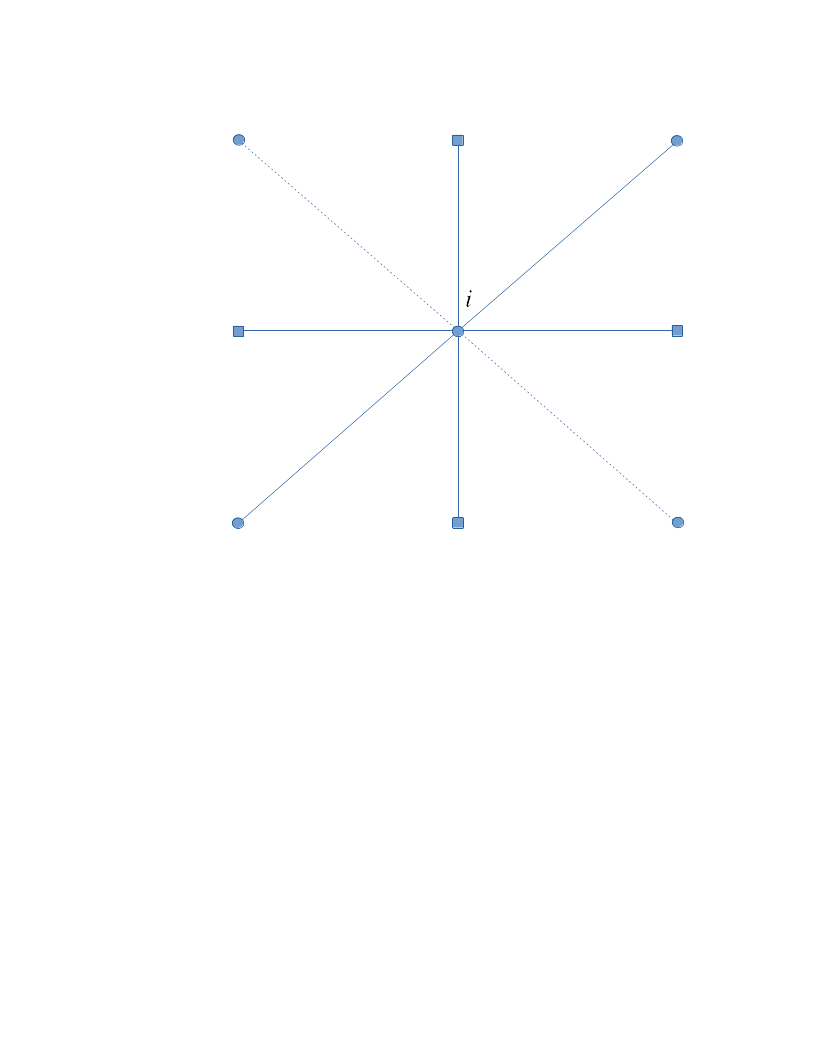
\includegraphics[width=0.5\textwidth]{../figures/interpStencil} % TODO fix all figures
\end{center}
\end{frame}

% Slide
\begin{frame}{Interpolation}
\begin{block}{Classical interpolation formula}
\bit
\item Strongly connected C-points form the interpolatory set
\item Rather than disregard F-F connections, collapse their values to the interpolation stencil
\eit
\end{block}
\begin{center}
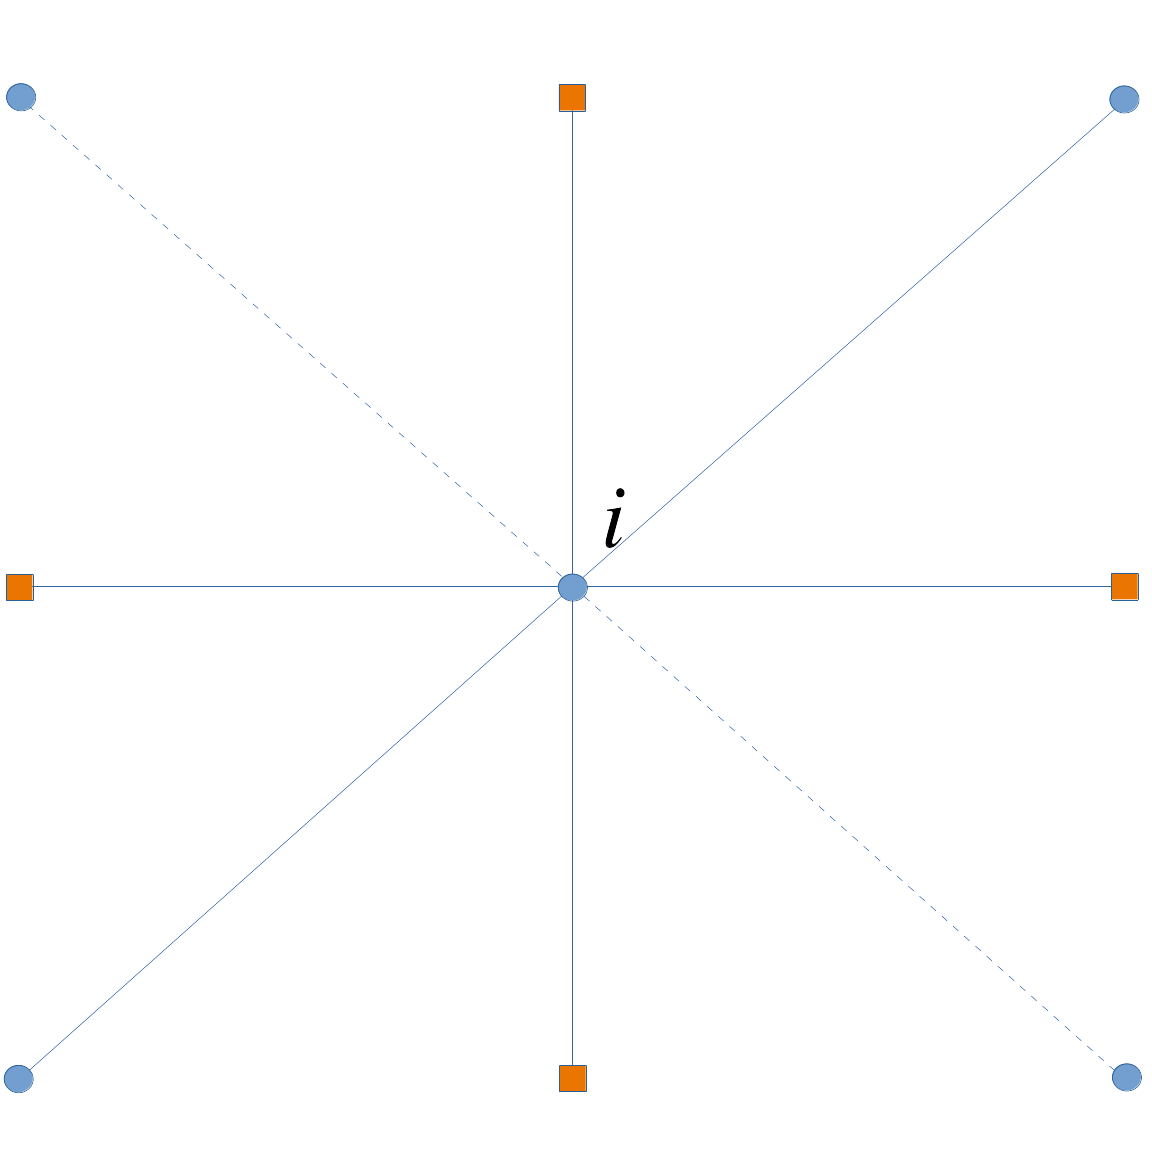
\includegraphics[width=0.5\textwidth]{../figures/interpStencilCpts}
\end{center}
\end{frame}

% Slide
\begin{frame}{Interpolation}
\begin{block}{Classical interpolation formula}
\bit
\item Weakly connected F-points are added to the diagonal
\item Assume $e_i\approx e_j$ for $j\in D^w_i$
\eit
\end{block}
\begin{center}
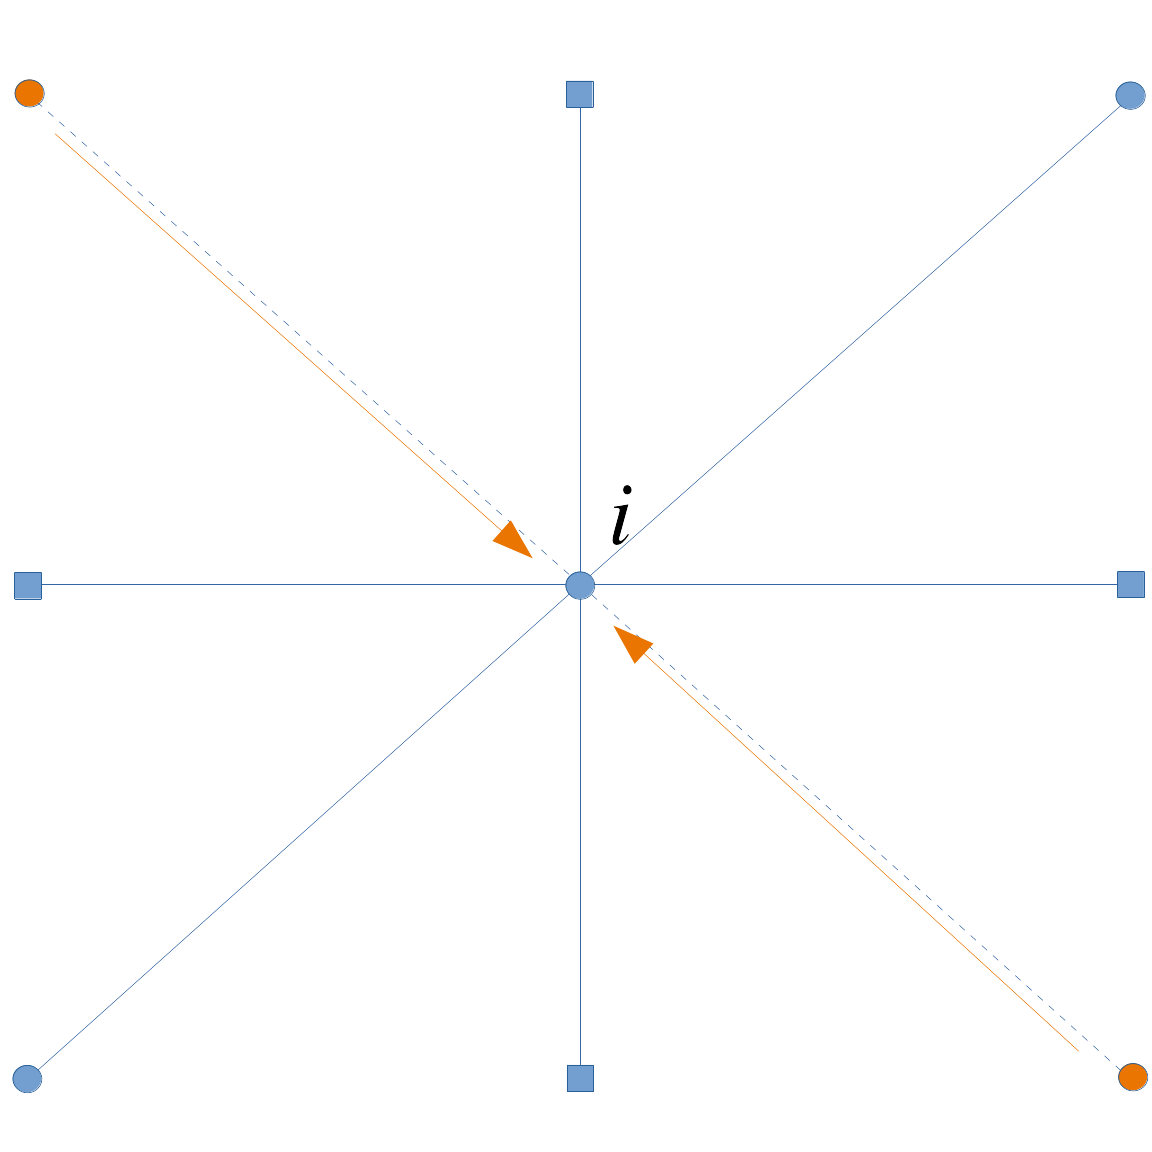
\includegraphics[width=0.5\textwidth]{../figures/interpStencilWeakF}
\end{center}
\end{frame}

% Slide
\begin{frame}{Interpolation}
\begin{block}{Classical interpolation formula}
\eq{
   a_{i,i} e_i = - \sum_{j\in C_i} a_{i,j}e_j - \sum_{j\in D^s_i} a_{i,j}e_j - \sum_{j\in D^w_i} a_{i,j}e_j \\
   (a_{i,i} + \sum_{j\in D^w_i} a_{i,j}) e_i = - \sum_{j\in C_i} a_{i,j}e_j - \sum_{j\in D^s_i} a_{i,j}e_j
}
\end{block}
\begin{center}
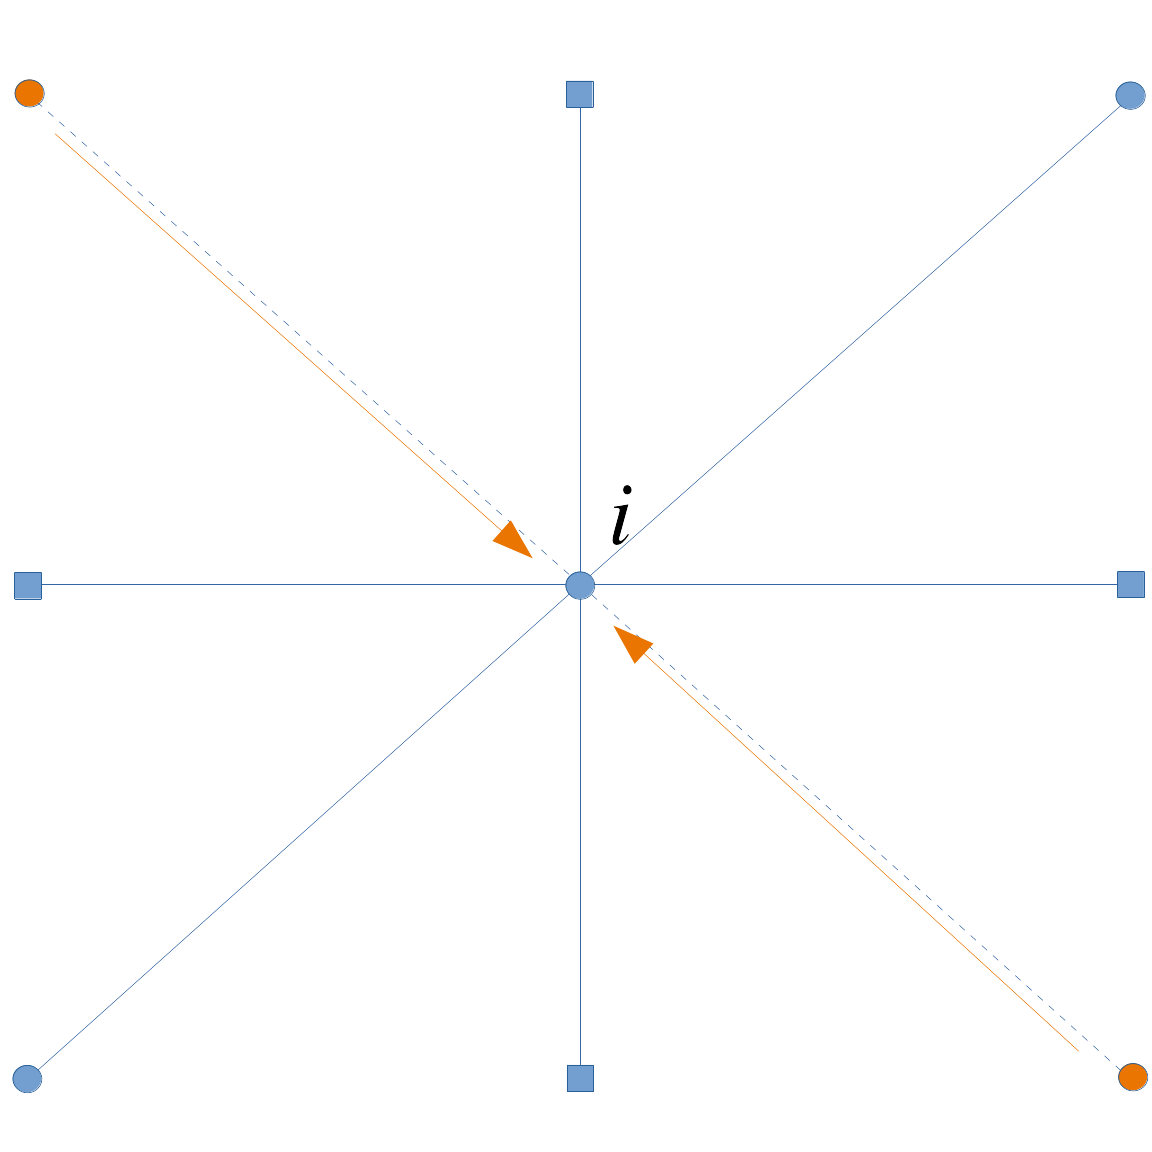
\includegraphics[width=0.5\textwidth]{../figures/interpStencilWeakF}
\end{center}
\end{frame}

% Slide
\begin{frame}{Interpolation}
\begin{block}{Classical interpolation formula}
\bit
\item Could do something similar with strong F-F connections
\item Practice has shown better results collapsing these values to the C-points
\eit
\end{block}
\begin{center}
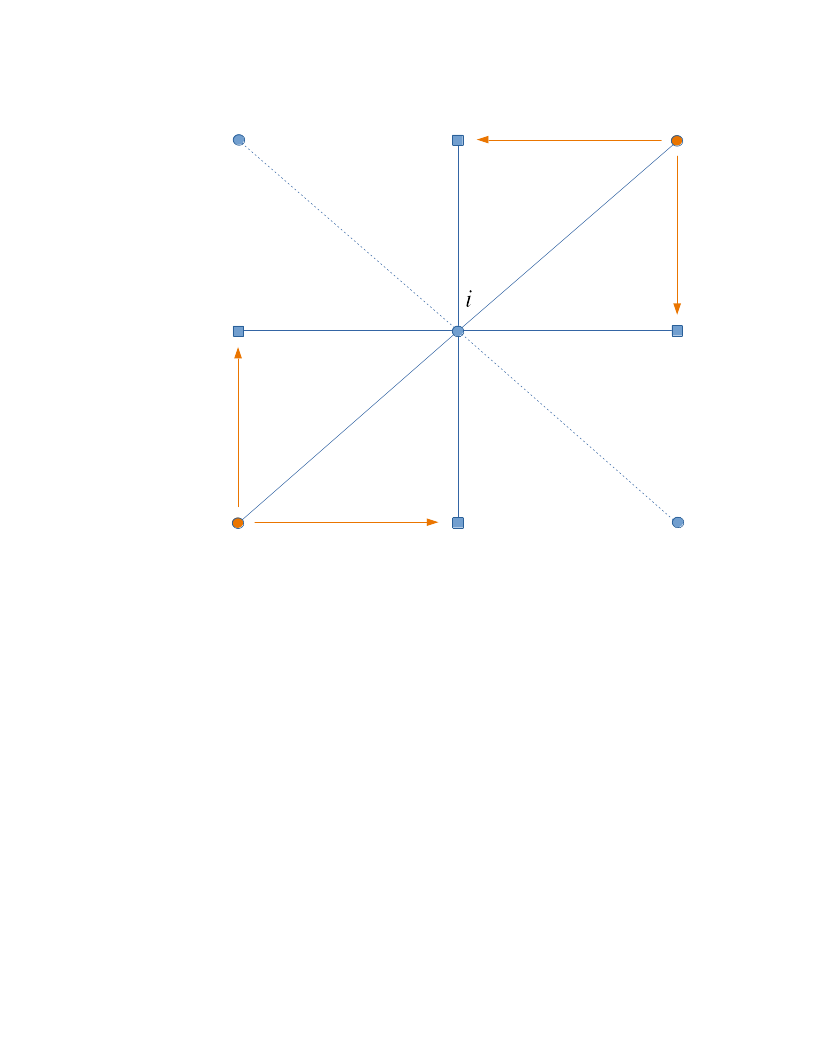
\includegraphics[width=0.5\textwidth]{../figures/interpStencilStrongF}
\end{center}
\end{frame}

% Slide
\begin{frame}{Interpolation}
\begin{block}{Classical interpolation formula}
\eq{
   e_j \approx \frac{\sum_{k \in C_i}a_{j,k}e_k}{\sum_{k \in C_i}a_{j,k}}
}
\end{block}
\begin{center}
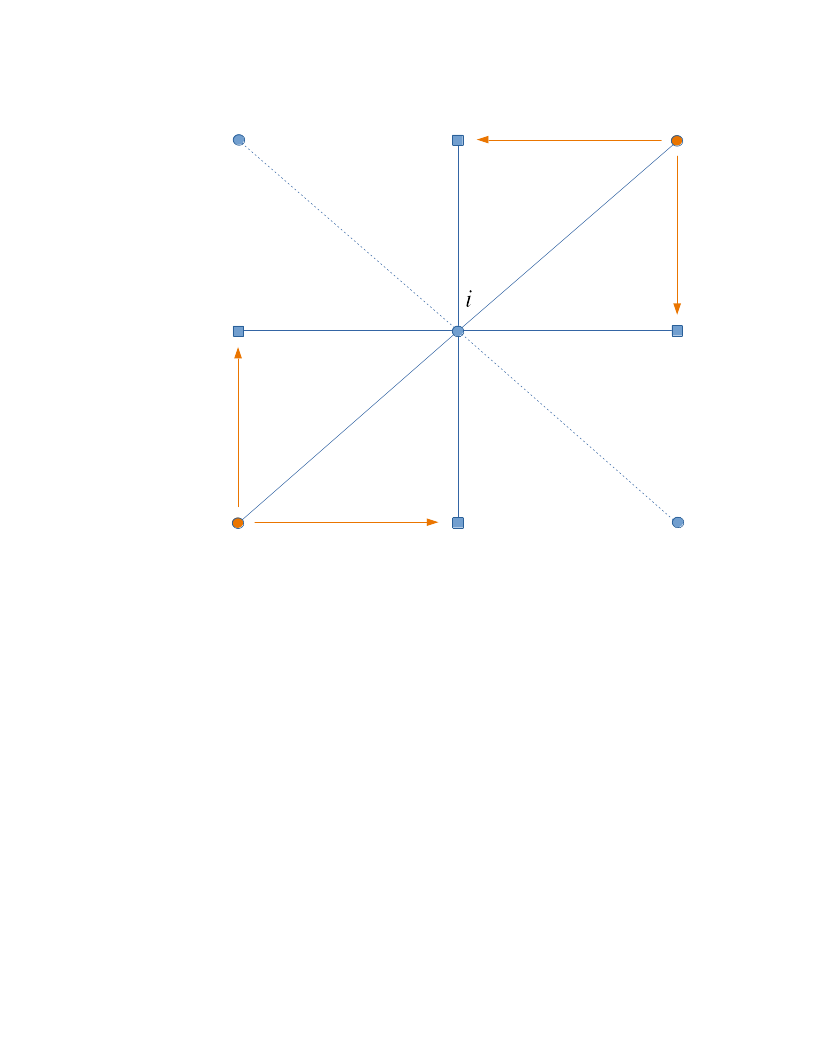
\includegraphics[width=0.5\textwidth]{../figures/interpStencilStrongF}
\end{center}
\end{frame}

% Slide
\begin{frame}{Interpolation}
\begin{block}{Classical interpolation formula}
\eq{
   &(a_{i,i} + \sum_{j\in D^w_i} a_{i,j}) e_i = - \sum_{j\in C_i} a_{i,j}e_j - \sum_{j\in D^s_i} a_{i,j}e_j \\
   &(a_{i,i} + \sum_{j\in D^w_i} a_{i,j}) e_i = - \sum_{j\in C_i} a_{i,j}e_j - \sum_{j\in D^s_i} a_{i,j}\frac{\sum_{k \in C_i}a_{j,k}e_k}{\sum_{k \in C_i}a_{j,k}}
}
\end{block}
\begin{center}
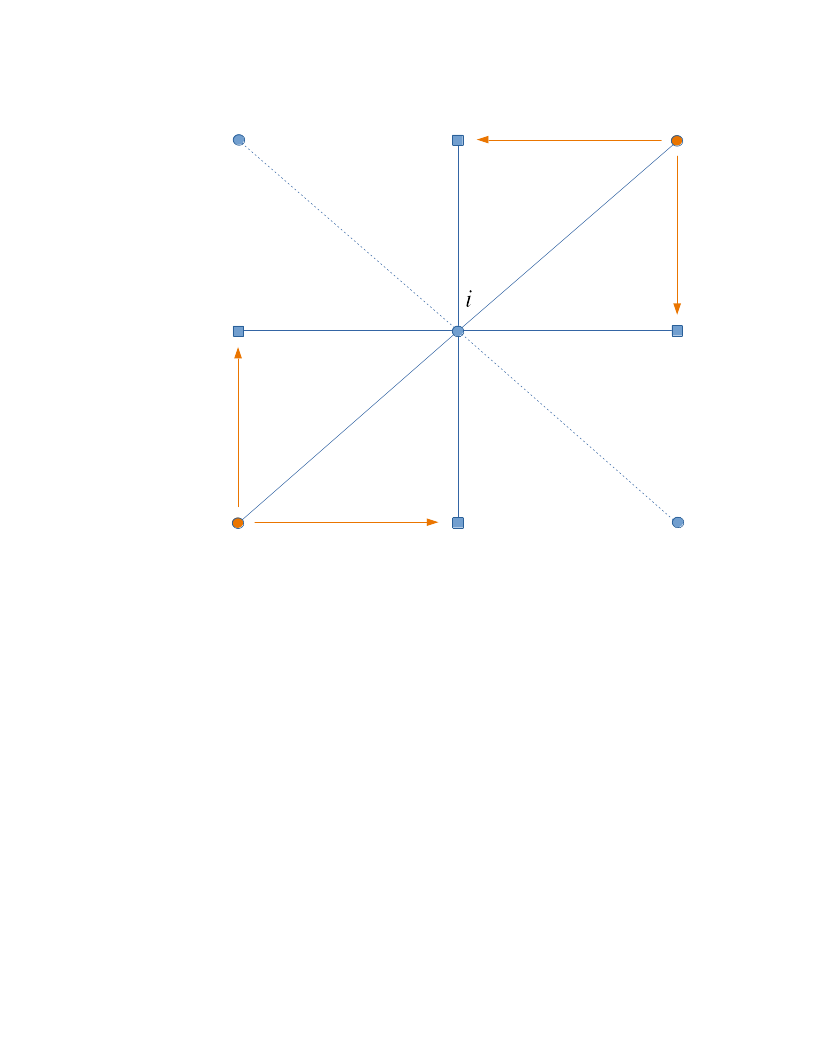
\includegraphics[width=0.5\textwidth]{../figures/interpStencilStrongF}
\end{center}
\end{frame}

% Slide
\begin{frame}{Interpolation}
\begin{block}{Classical interpolation formula}
\bit
\item Final interpolation formula
\eq{
   w_{i,j} = -\frac{a_{i,j} + \sum_{m\in D^s_i} \left( \frac{a_{i,m}a_{m,j}}{\sum_{k\in C_i} a_{m,k}} \right)}{a_ii + \sum_{n \in D^w_i} a_{i,j}}
}
\eit
\end{block}
\begin{center}
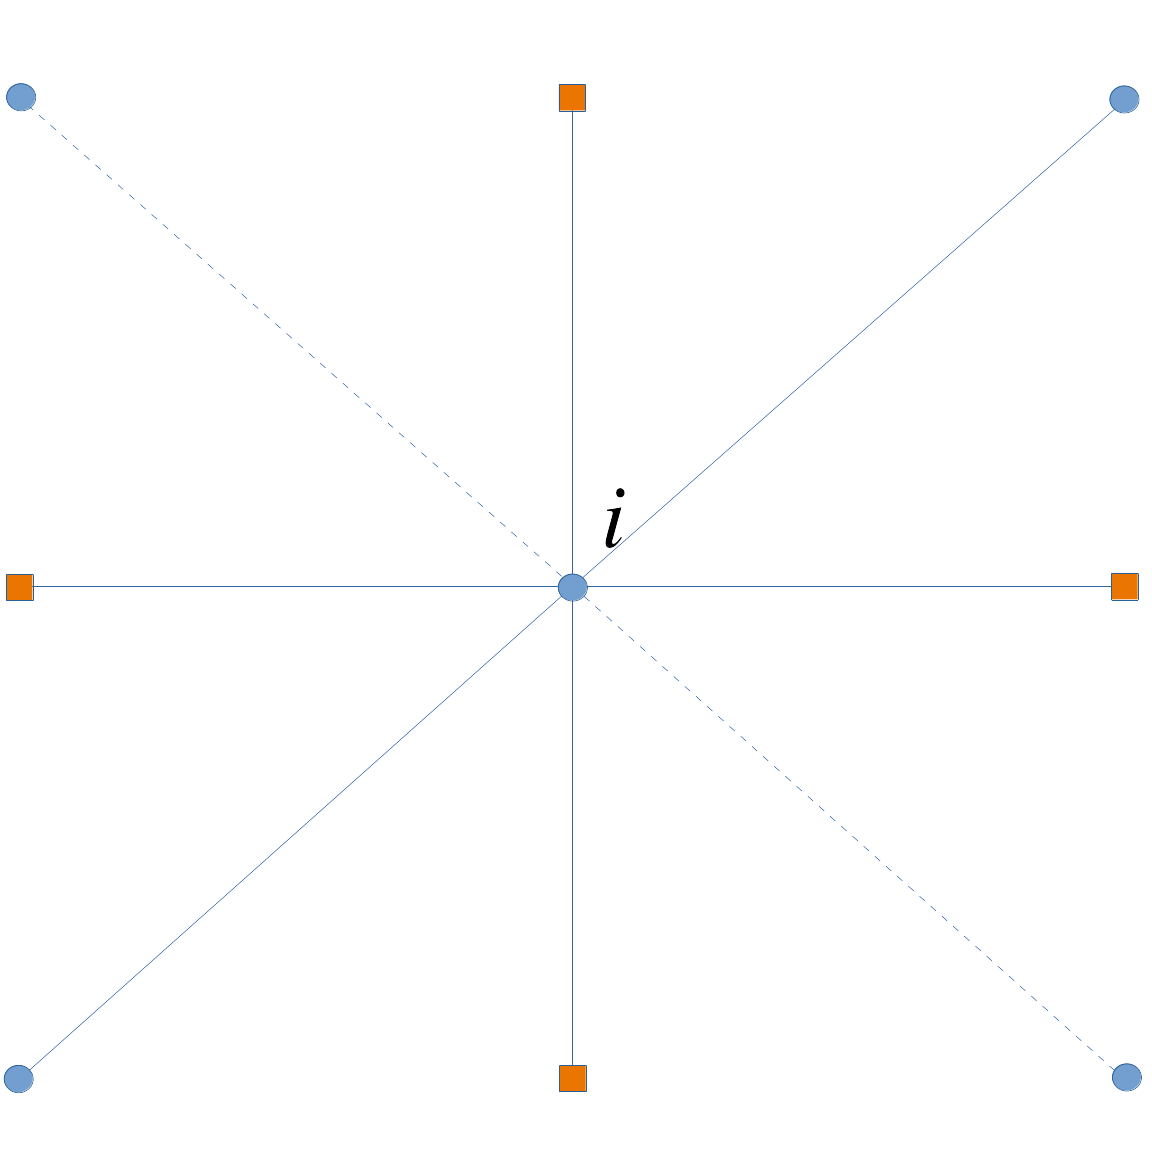
\includegraphics[width=0.5\textwidth]{../figures/interpStencilCpts}
\end{center}
\end{frame}

% Slide
\begin{frame}{Interpolation}
\begin{block}{Classical interpolation formula}
\bit
\item Final interpolation formula
\eq{
   (P\mathbf{e})_i = \begin{cases}
   e_i, & i\in C \\
   \sum_{j\in C_i} w_{i,j}e_j, & i \in F
   \end{cases}
}
\eit
\end{block}
\begin{center}
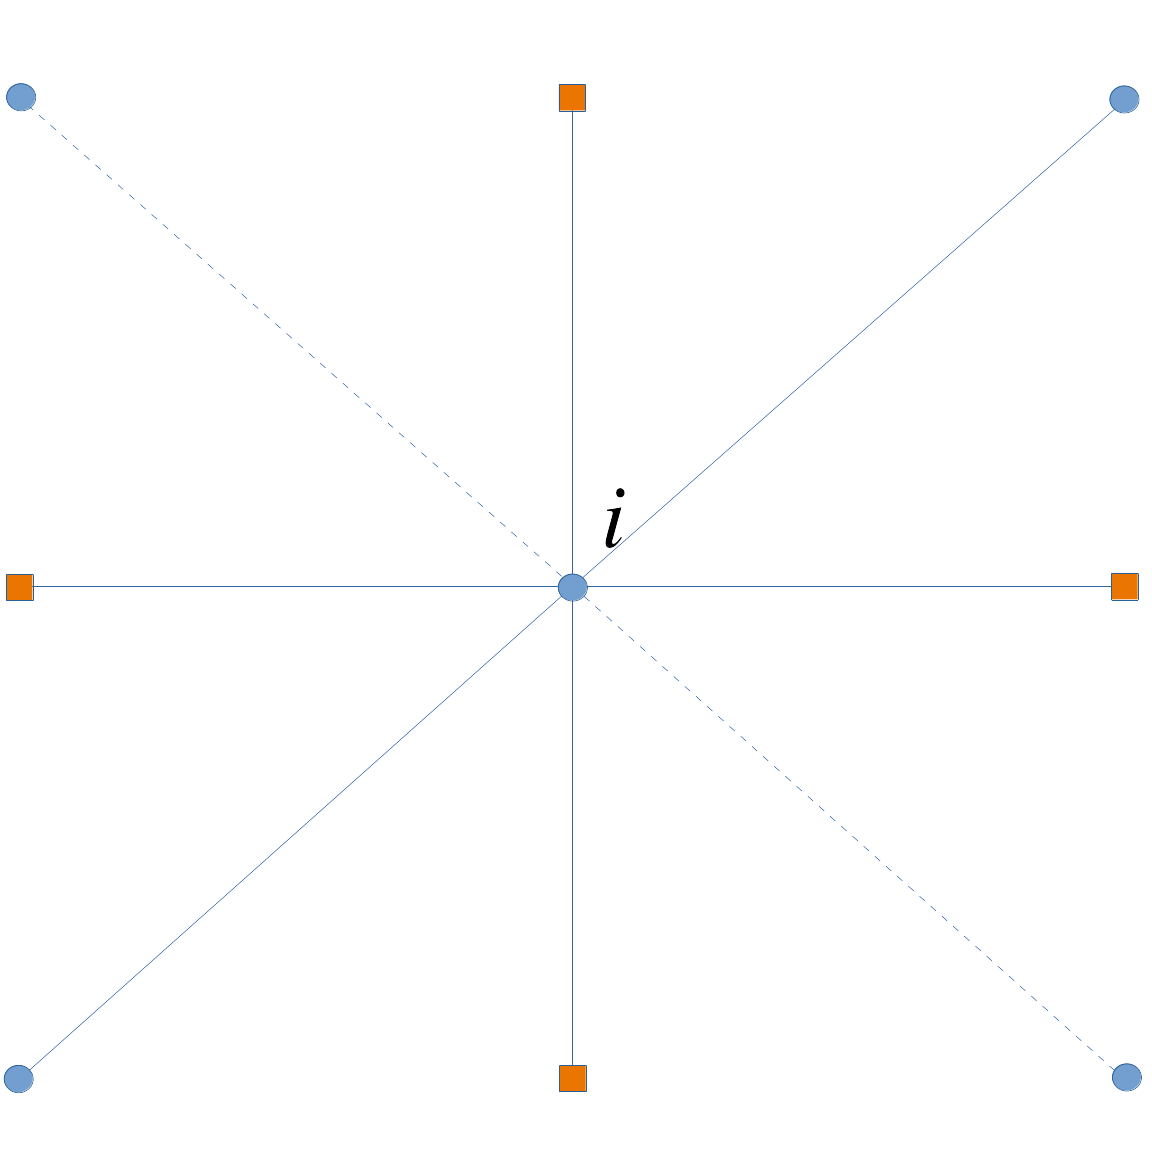
\includegraphics[width=0.5\textwidth]{../figures/interpStencilCpts}
\end{center}
\end{frame}

% Slide
\begin{frame}{Interpolation}
\begin{block}{Notes on classical interpolation}
\bit
\item This is just one way of calculating interpolation weights
\item There are many other approaches
\item Active area of research for more difficult problems
\eit
\end{block}
\end{frame}

%%%%%%%%%%%%%%%%%%%%%%%%%%%%%%%%%%%%%%%%%%%%%%%%%%%%%%%%%%%%%%%%%%%%%%%%%%%%%%%%

\section{Coarsening}

% Slide
\begin{frame}{Coarsening}
\begin{block}{Requirements for the coarse grid}
\bit
\item Accurate approximate represention of smooth error from the fine grid
\item Accurate interpolation from coarse to fine grid
\item Significantly fewer points than the fine grid
\eit
\end{block}
\end{frame}

% Slide
\begin{frame}{Coarsening}
\begin{block}{Coarse grid heuristics}
\bit
\item Let $S_i$ be the set of points that strongly influence $i$
\item Let $C_i$ be the interpolatory set for F-point, $i$
\item Then the coarse grid should attempt to ensure the following heuristics:
\begin{enumerate}
\item For each F-point, $i$, every point $j\in S_i$ is either in $C_i$ or strongly depends on at least one point in $C_i$
\item The set of C-points is a maximal subset such that no C-point strongly depends on another C-point.
\end{enumerate}
\eit
\end{block}
\end{frame}

% Slide
\begin{frame}{Coarsening}
\begin{block}{Coarse grid heuristics}
\bit
\item Heuristic 1 allows collapsing strong F-F connections to C-points in the interpolation stencil
\item Heuristic 2 controls the size of the coarse grid: large enough for good convergence but small enough to control computational work
\item Not always possible to enforce both heuristics
\eit
\end{block}
\end{frame}

% Slide
\begin{frame}{Coarsening}
\begin{block}{Coloring scheme}
\bit
\item Classical AMG selects the coarse grid using a coloring scheme
\item Proceeds in two passes 
\item First, ``high-quality" C-points are added following heuristic 2
\item Second, additional C-points are added to enforce heuristic 1
\eit
\end{block}
\end{frame}

% Slide
\begin{frame}{Coarsening}
\begin{block}{Coloring scheme}
\bit
\item High-quality C-points strongly influence lots of F-points
\item Let $S^T_i$ be the set of points that $i$ strongly influences and $\lambda_i = |S^T_i|$
\item First pass proceeds as follows:
\begin{enumerate}
\item Select a point, $i$, with maximum $\lambda_i$ and mark as C-point
\item Mark points $j\in S^T_i$ as F-points
\item Increment $\lambda_k$ for unmarked points $k\in S_j$ for each $j\in S^T_i$
\item Repeat
\end{enumerate}
\eit
\end{block}
\end{frame}

% Slide
\begin{frame}{Coarsening}
\only<1>{
\begin{center}
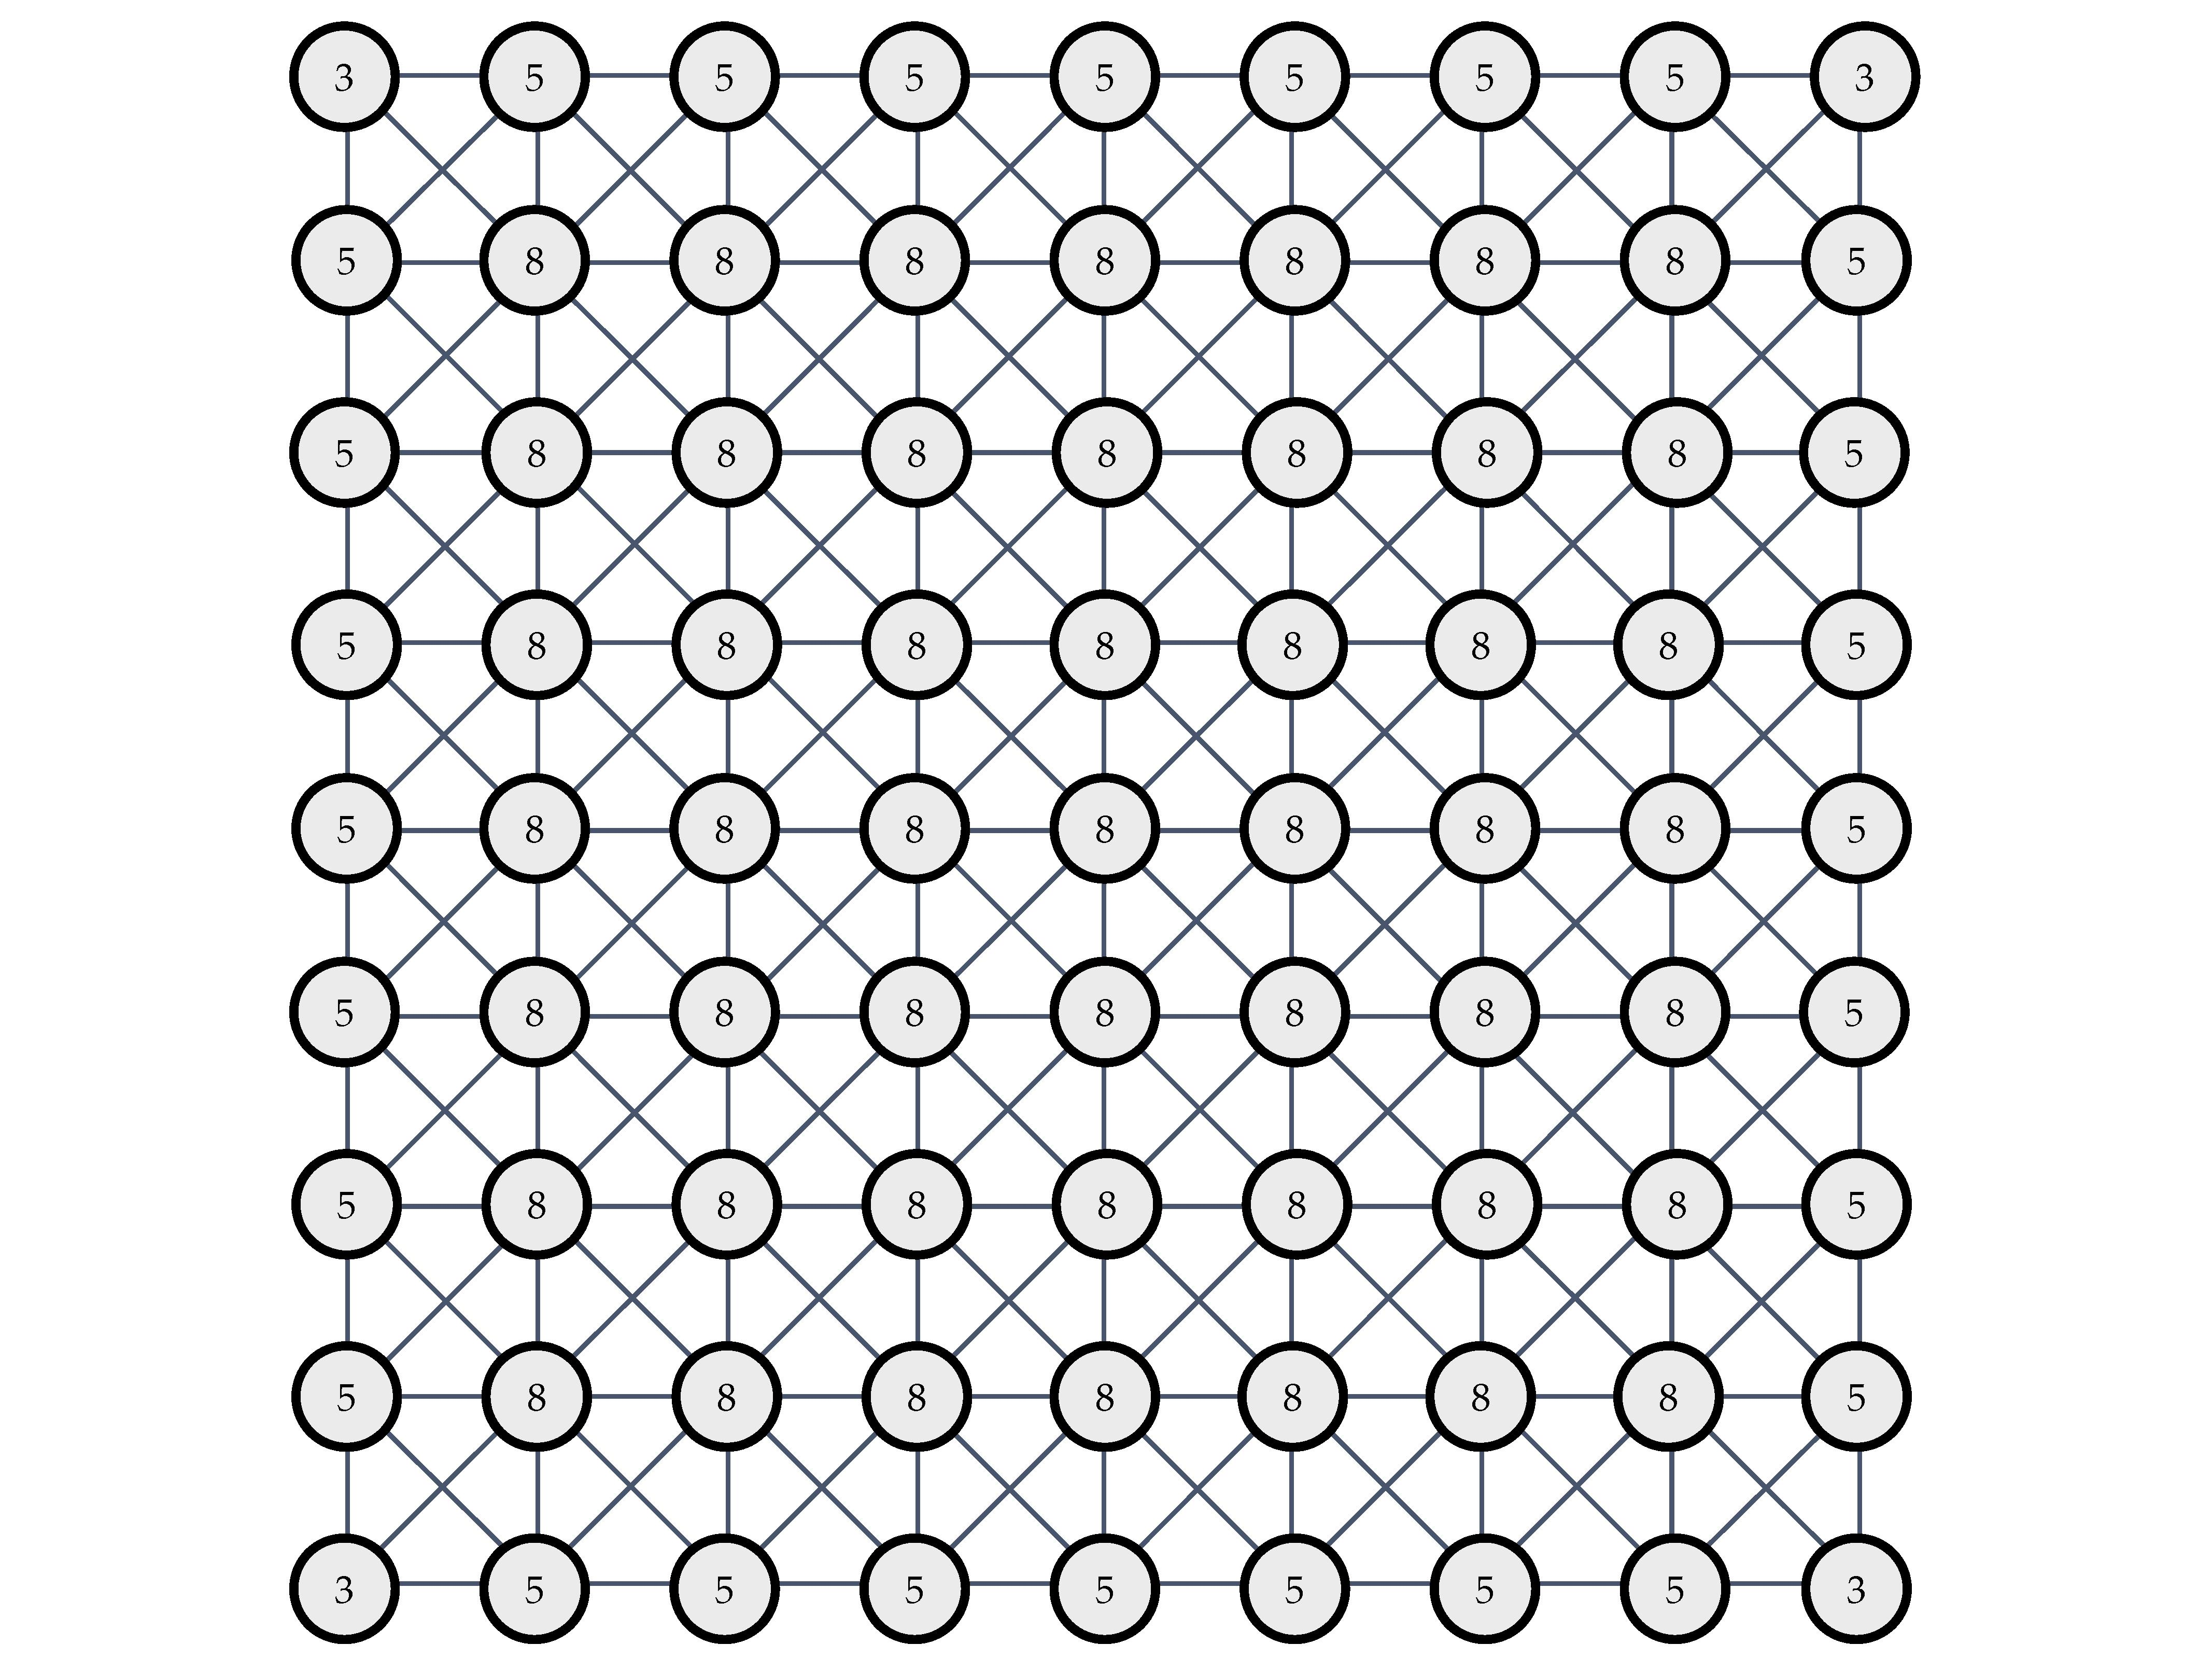
\includegraphics[width=0.7\textwidth]{../figures/amgCoarsening}
\end{center}}
\only<2>{
\begin{center}
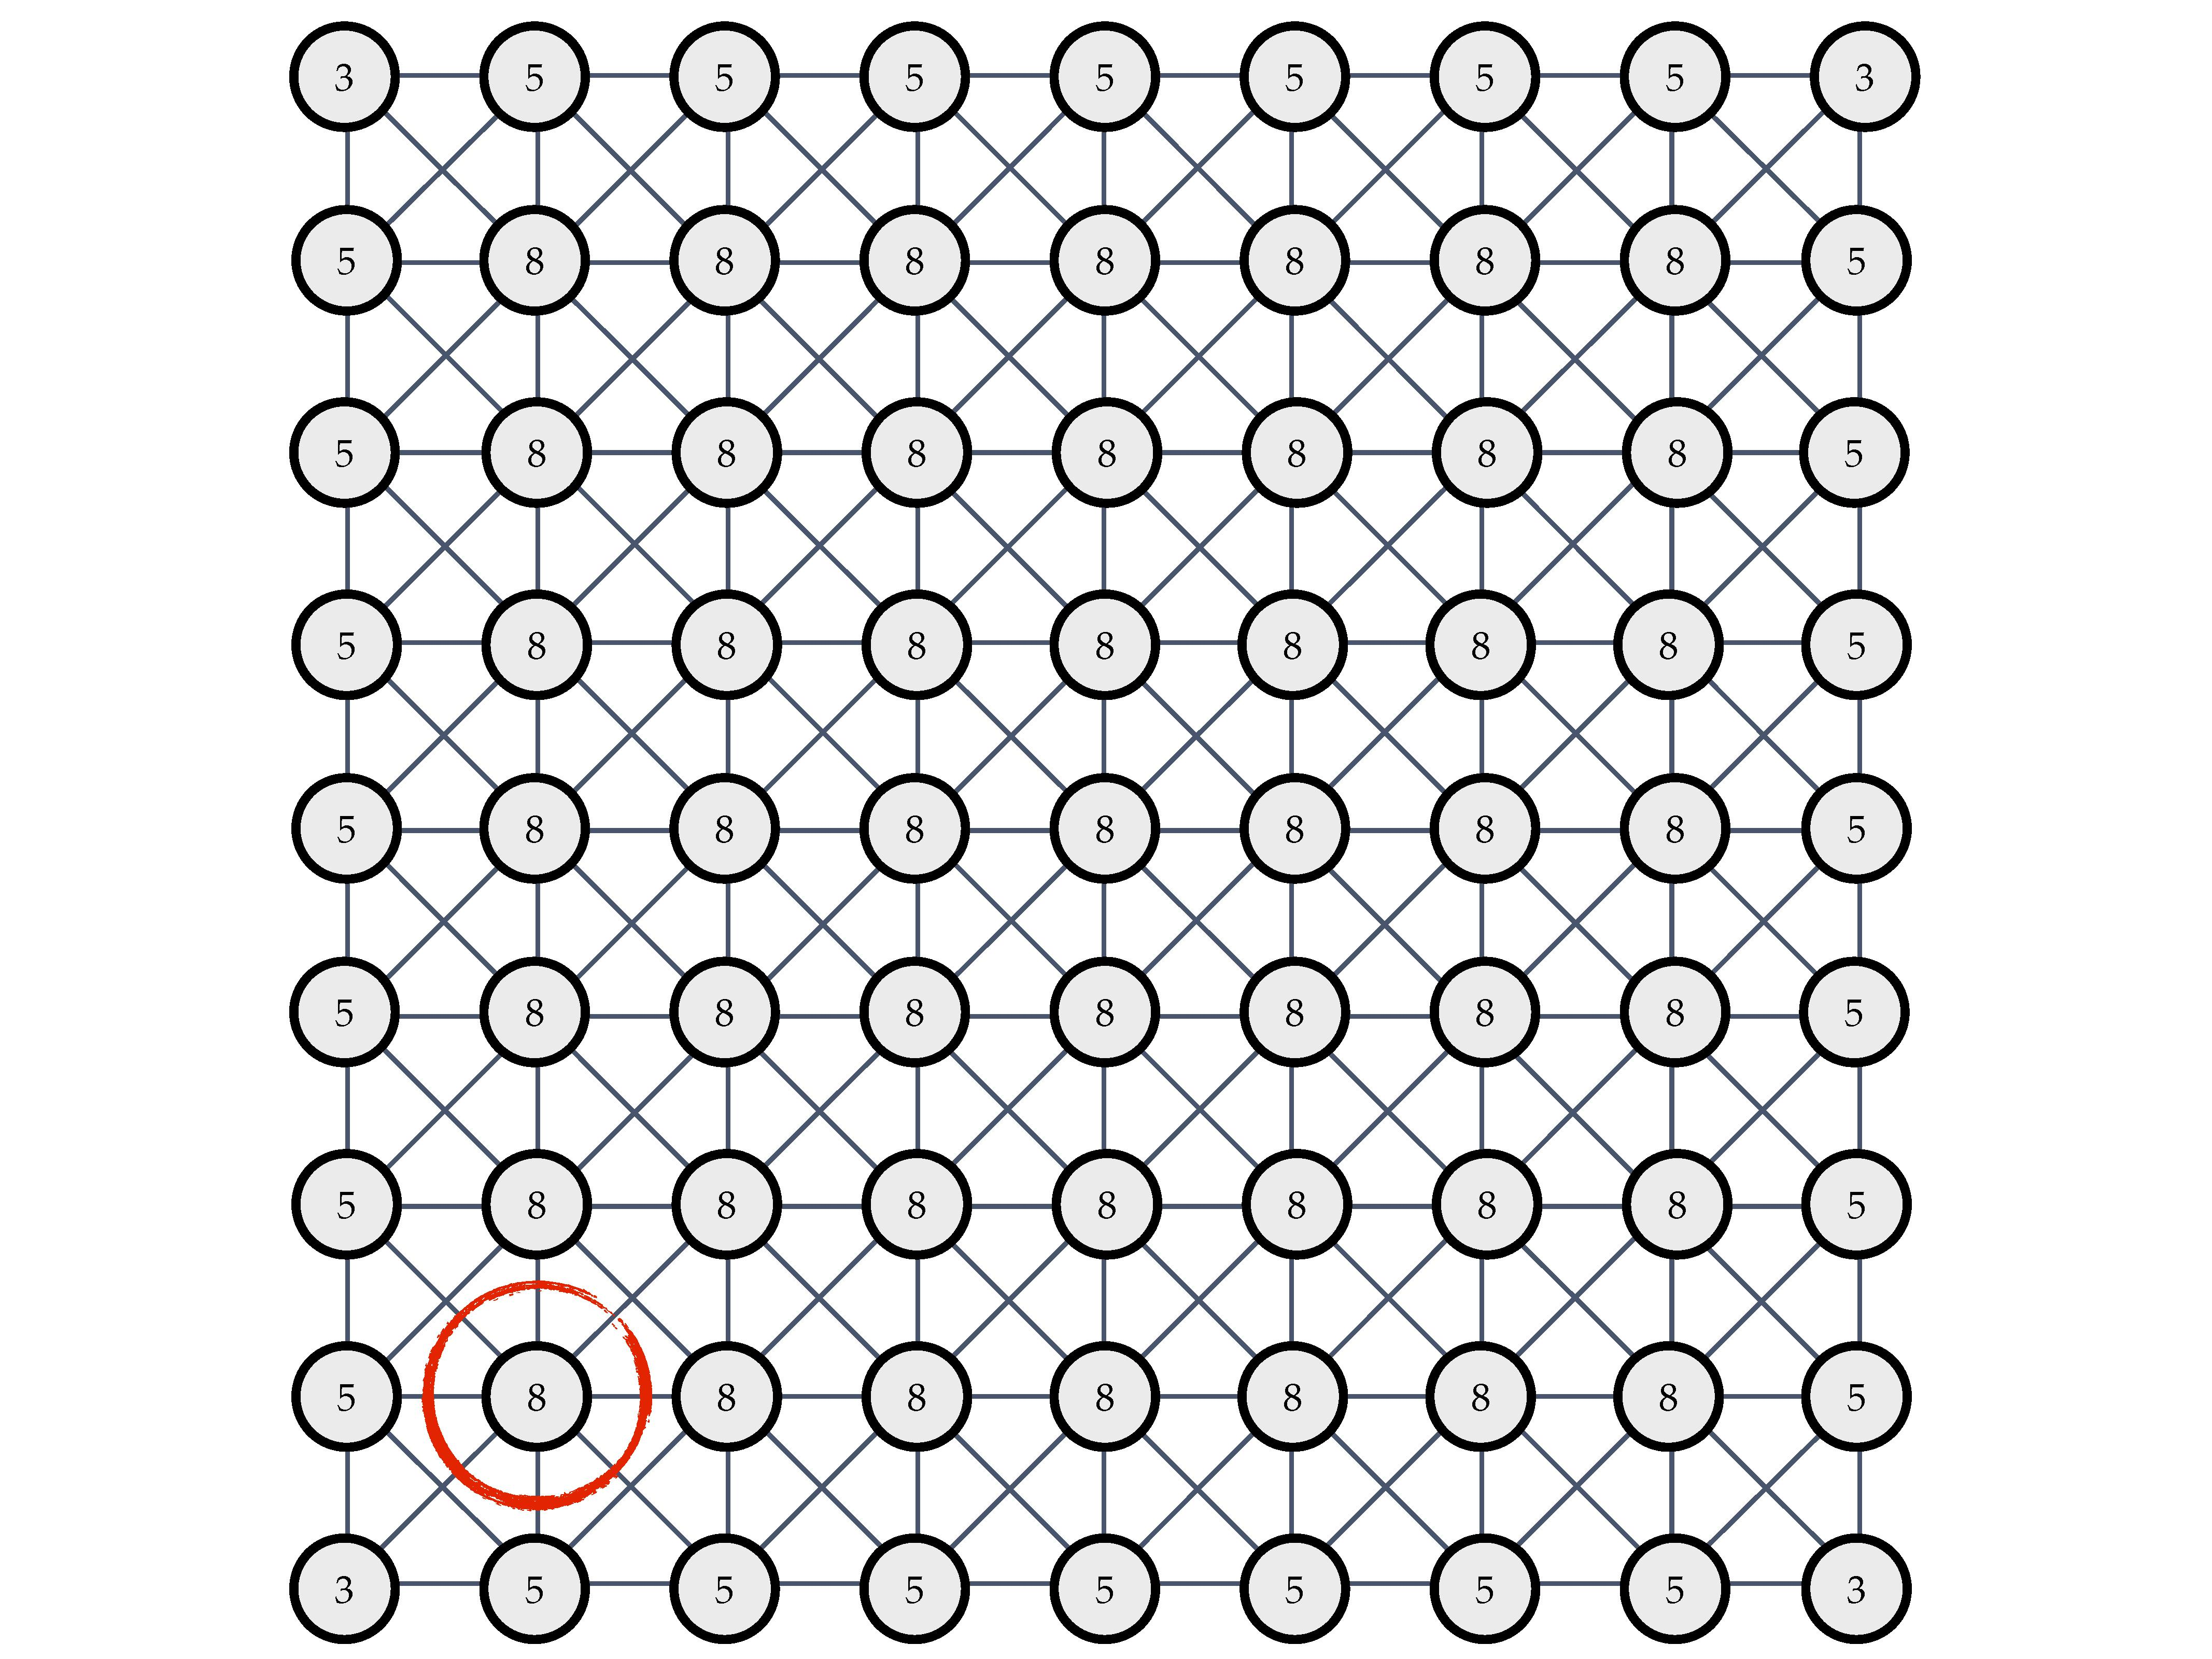
\includegraphics[width=0.7\textwidth]{../figures/amgCoarsening-2}
\end{center}}
\only<3>{
\begin{center}
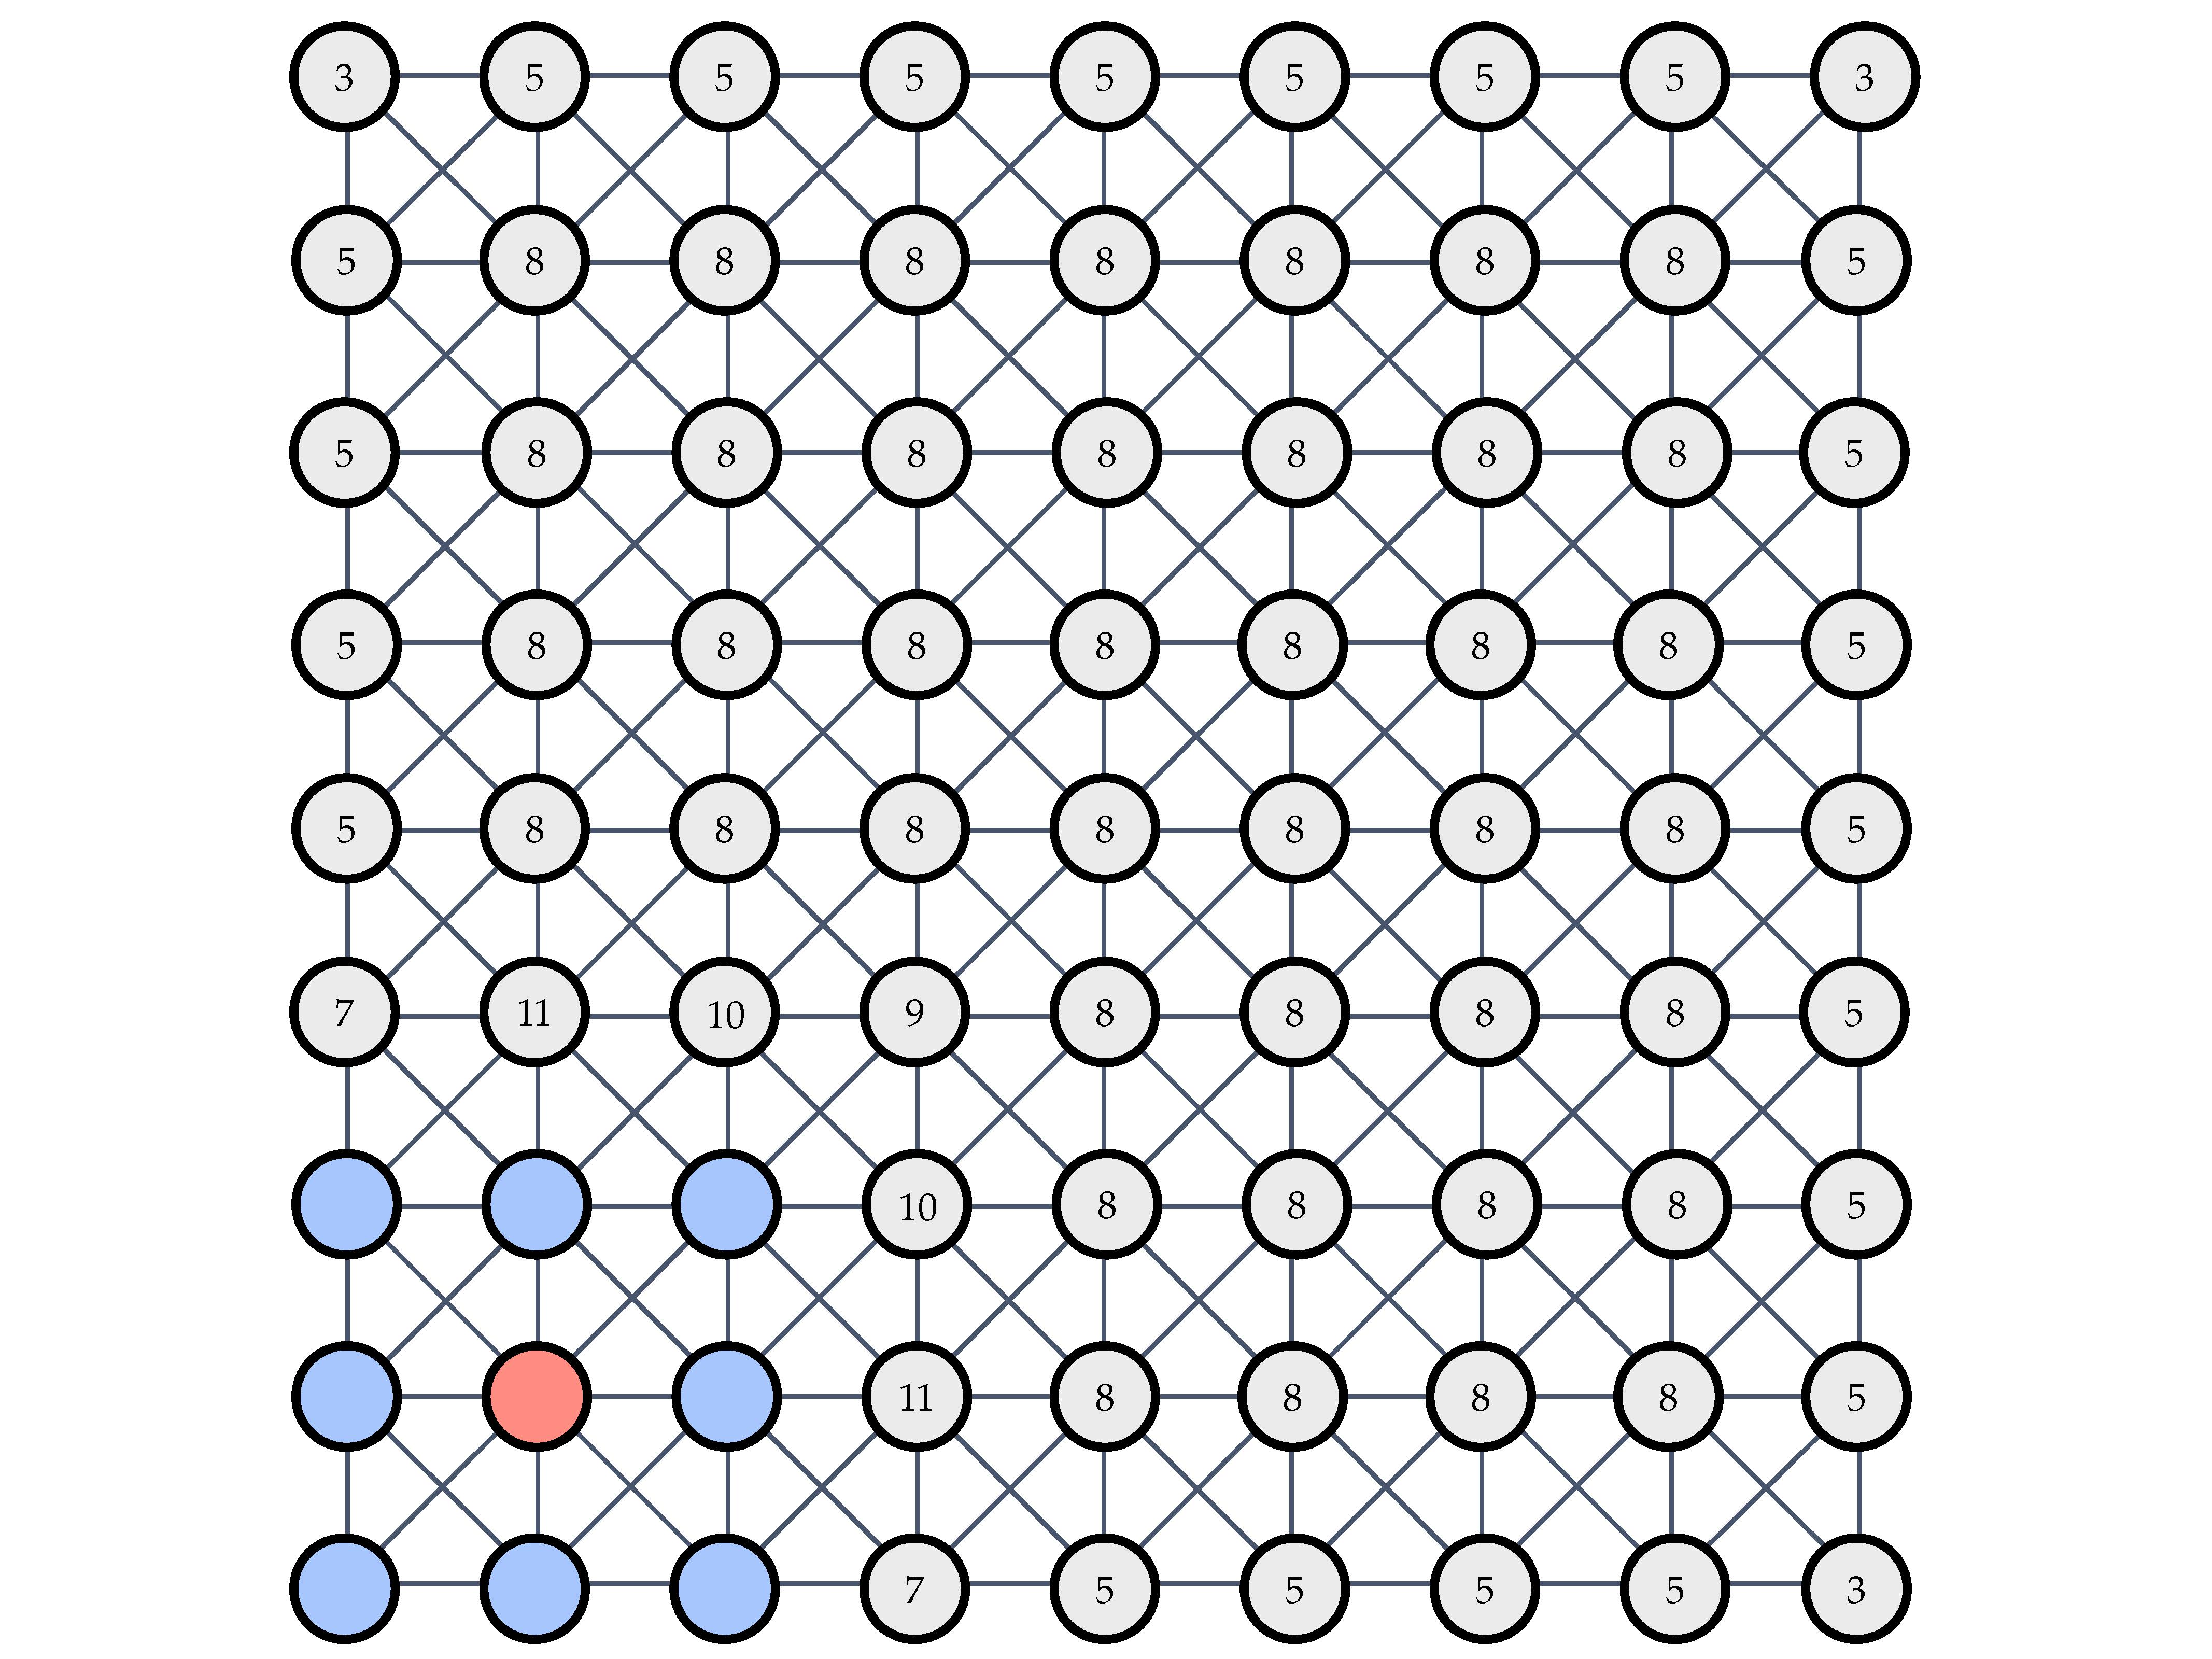
\includegraphics[width=0.7\textwidth]{../figures/amgCoarsening-3}
\end{center}}
\only<4>{
\begin{center}
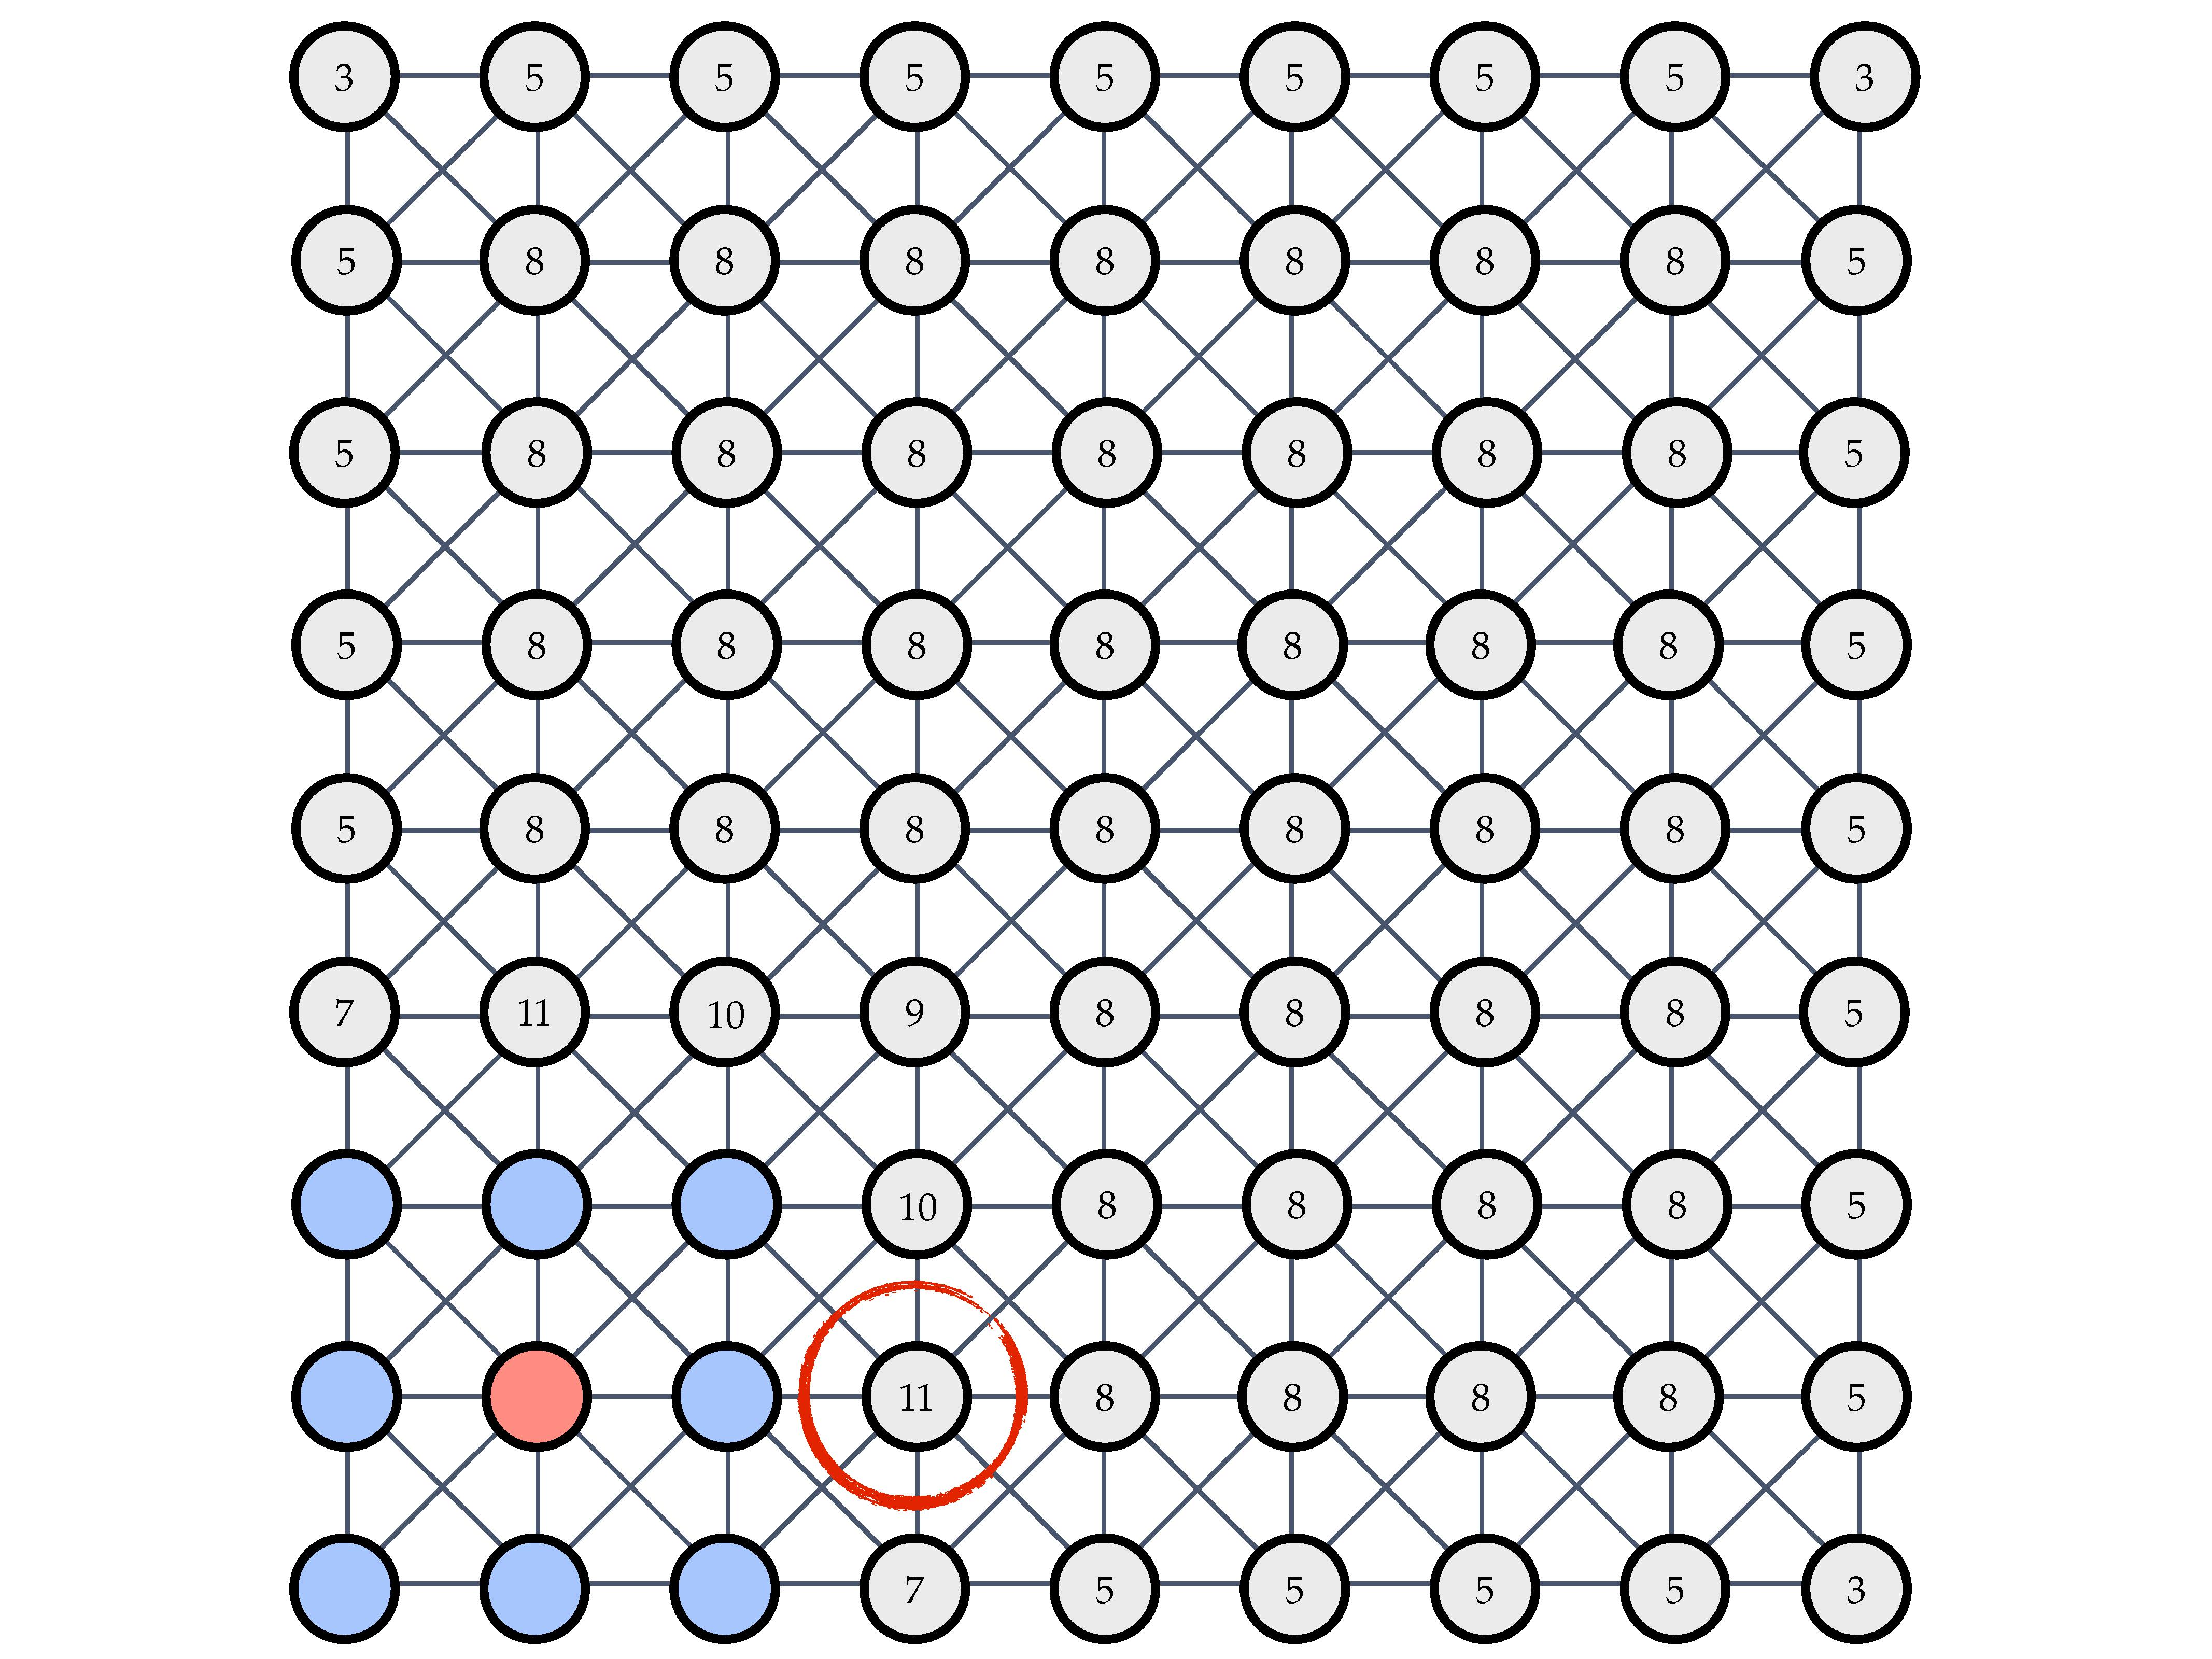
\includegraphics[width=0.7\textwidth]{../figures/amgCoarsening-4}
\end{center}}
\only<5>{
\begin{center}
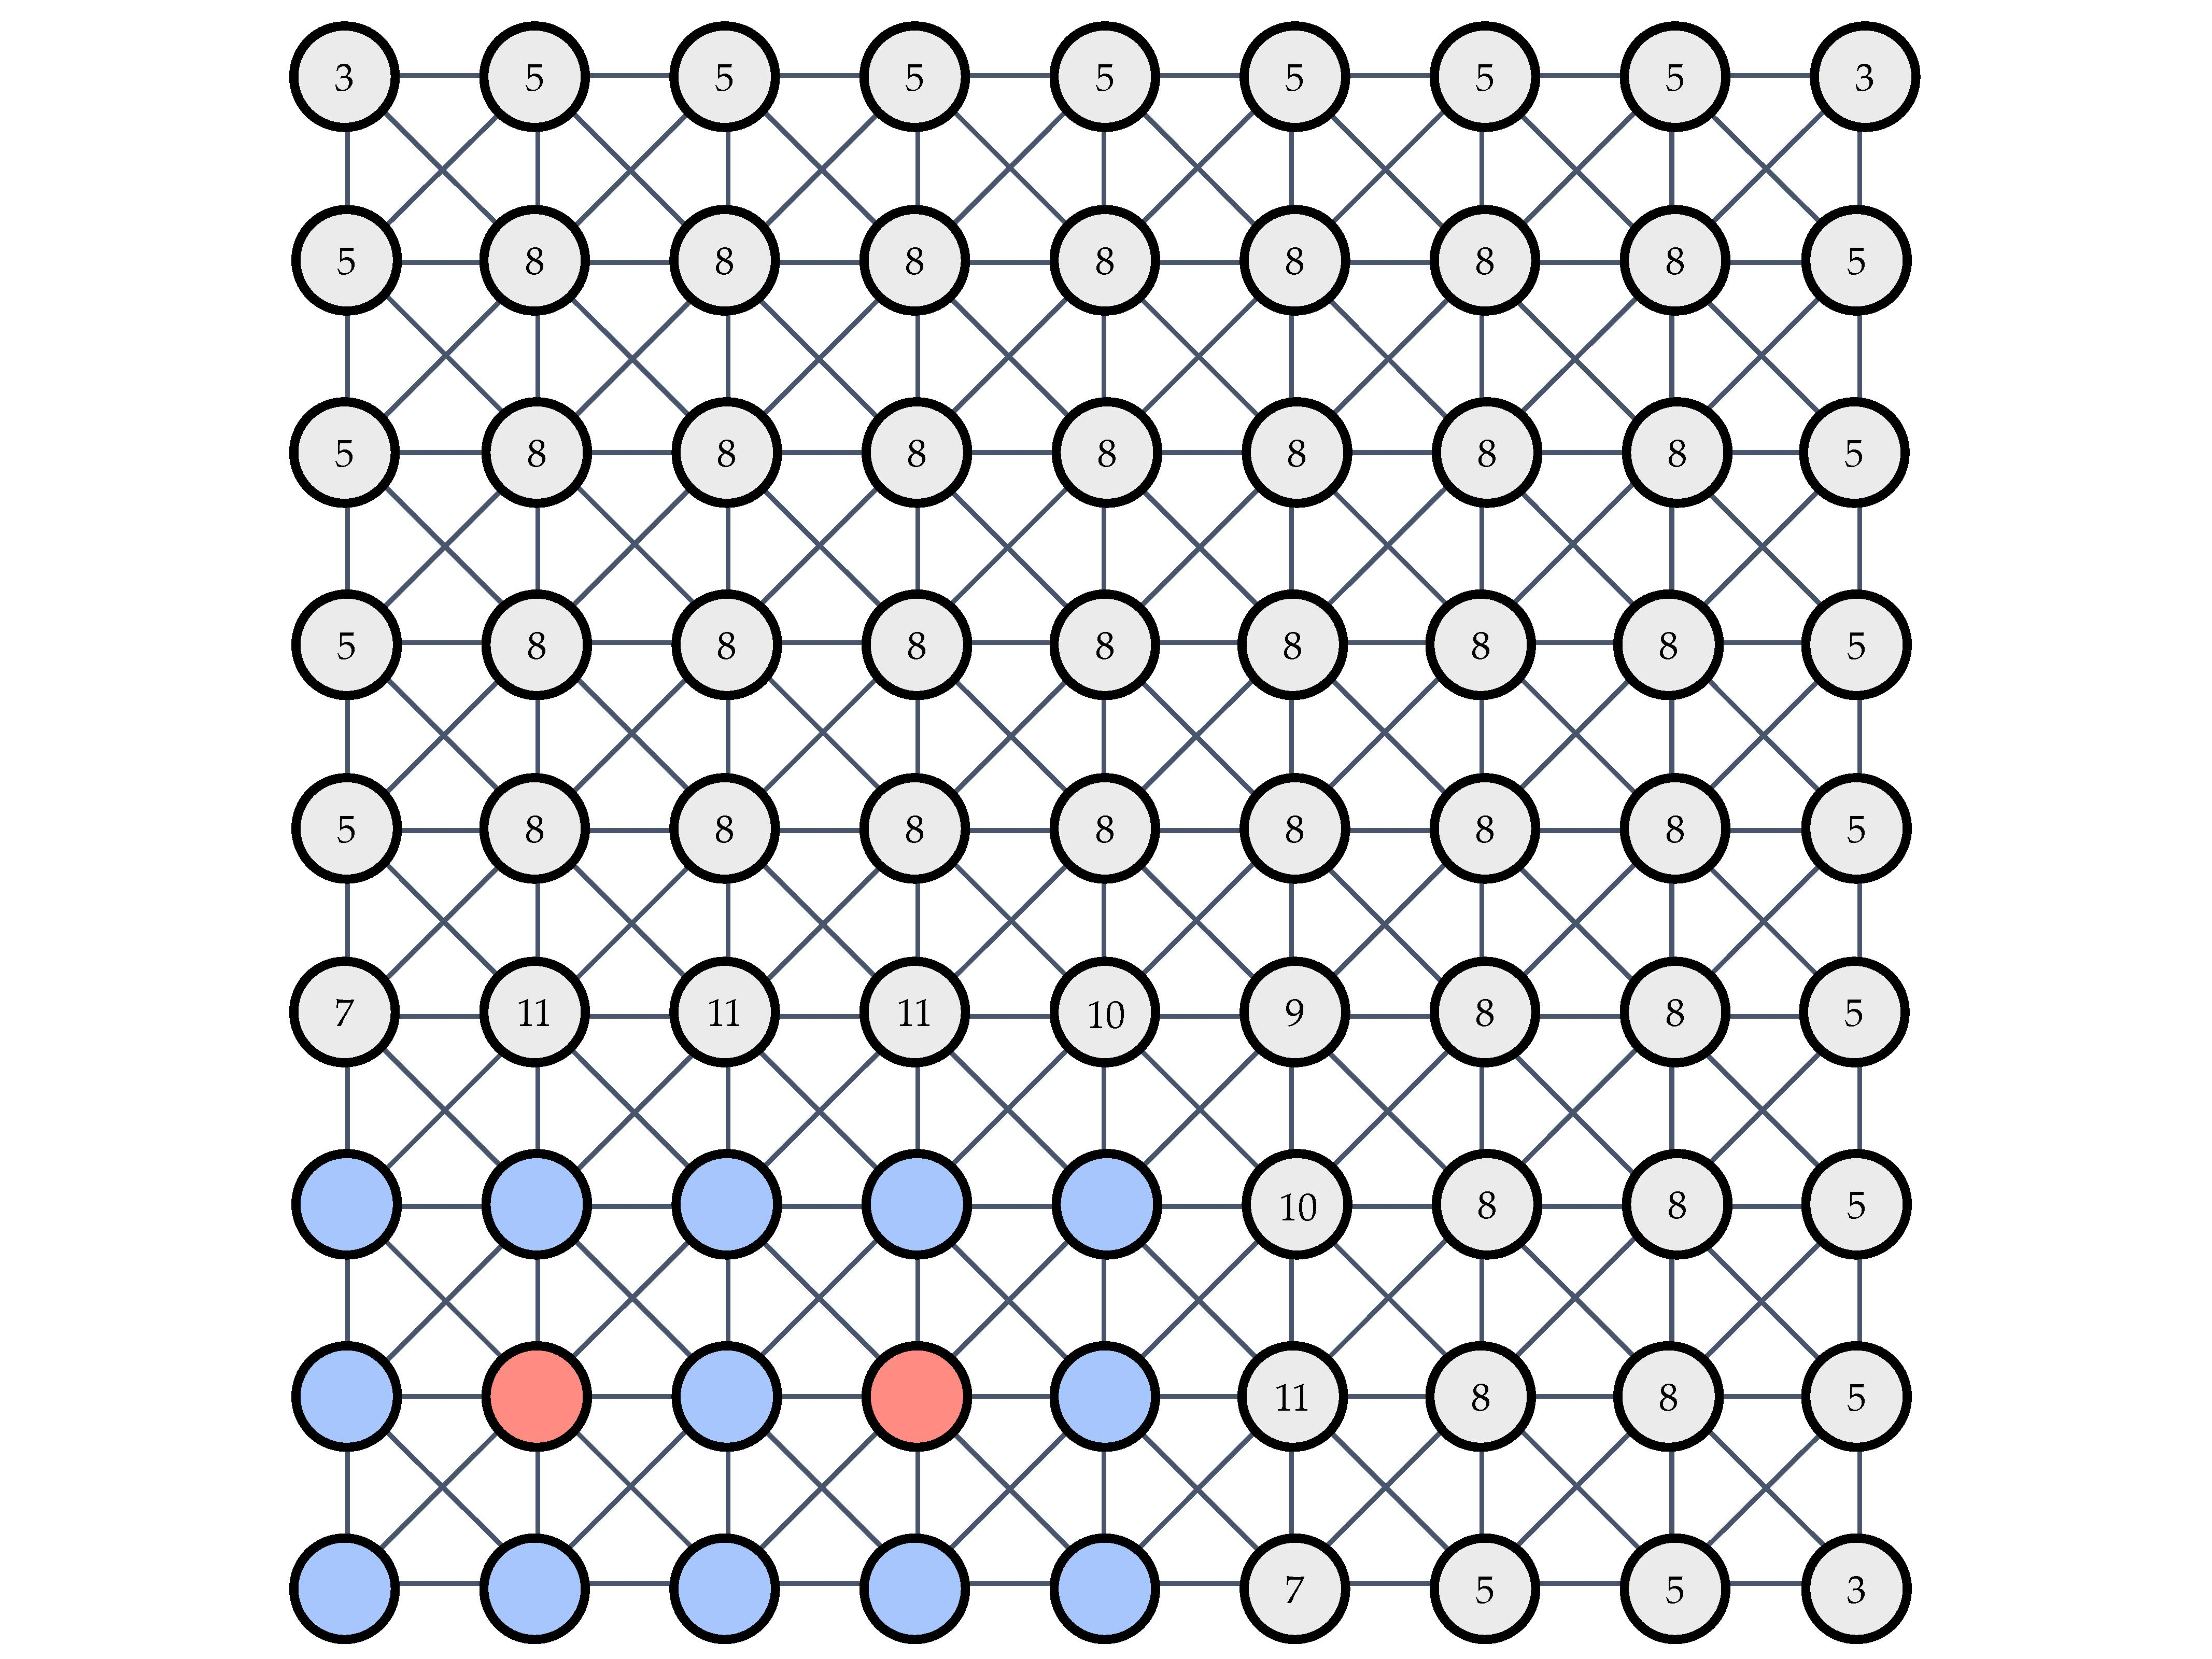
\includegraphics[width=0.7\textwidth]{../figures/amgCoarsening-5}
\end{center}}
\only<6>{
\begin{center}
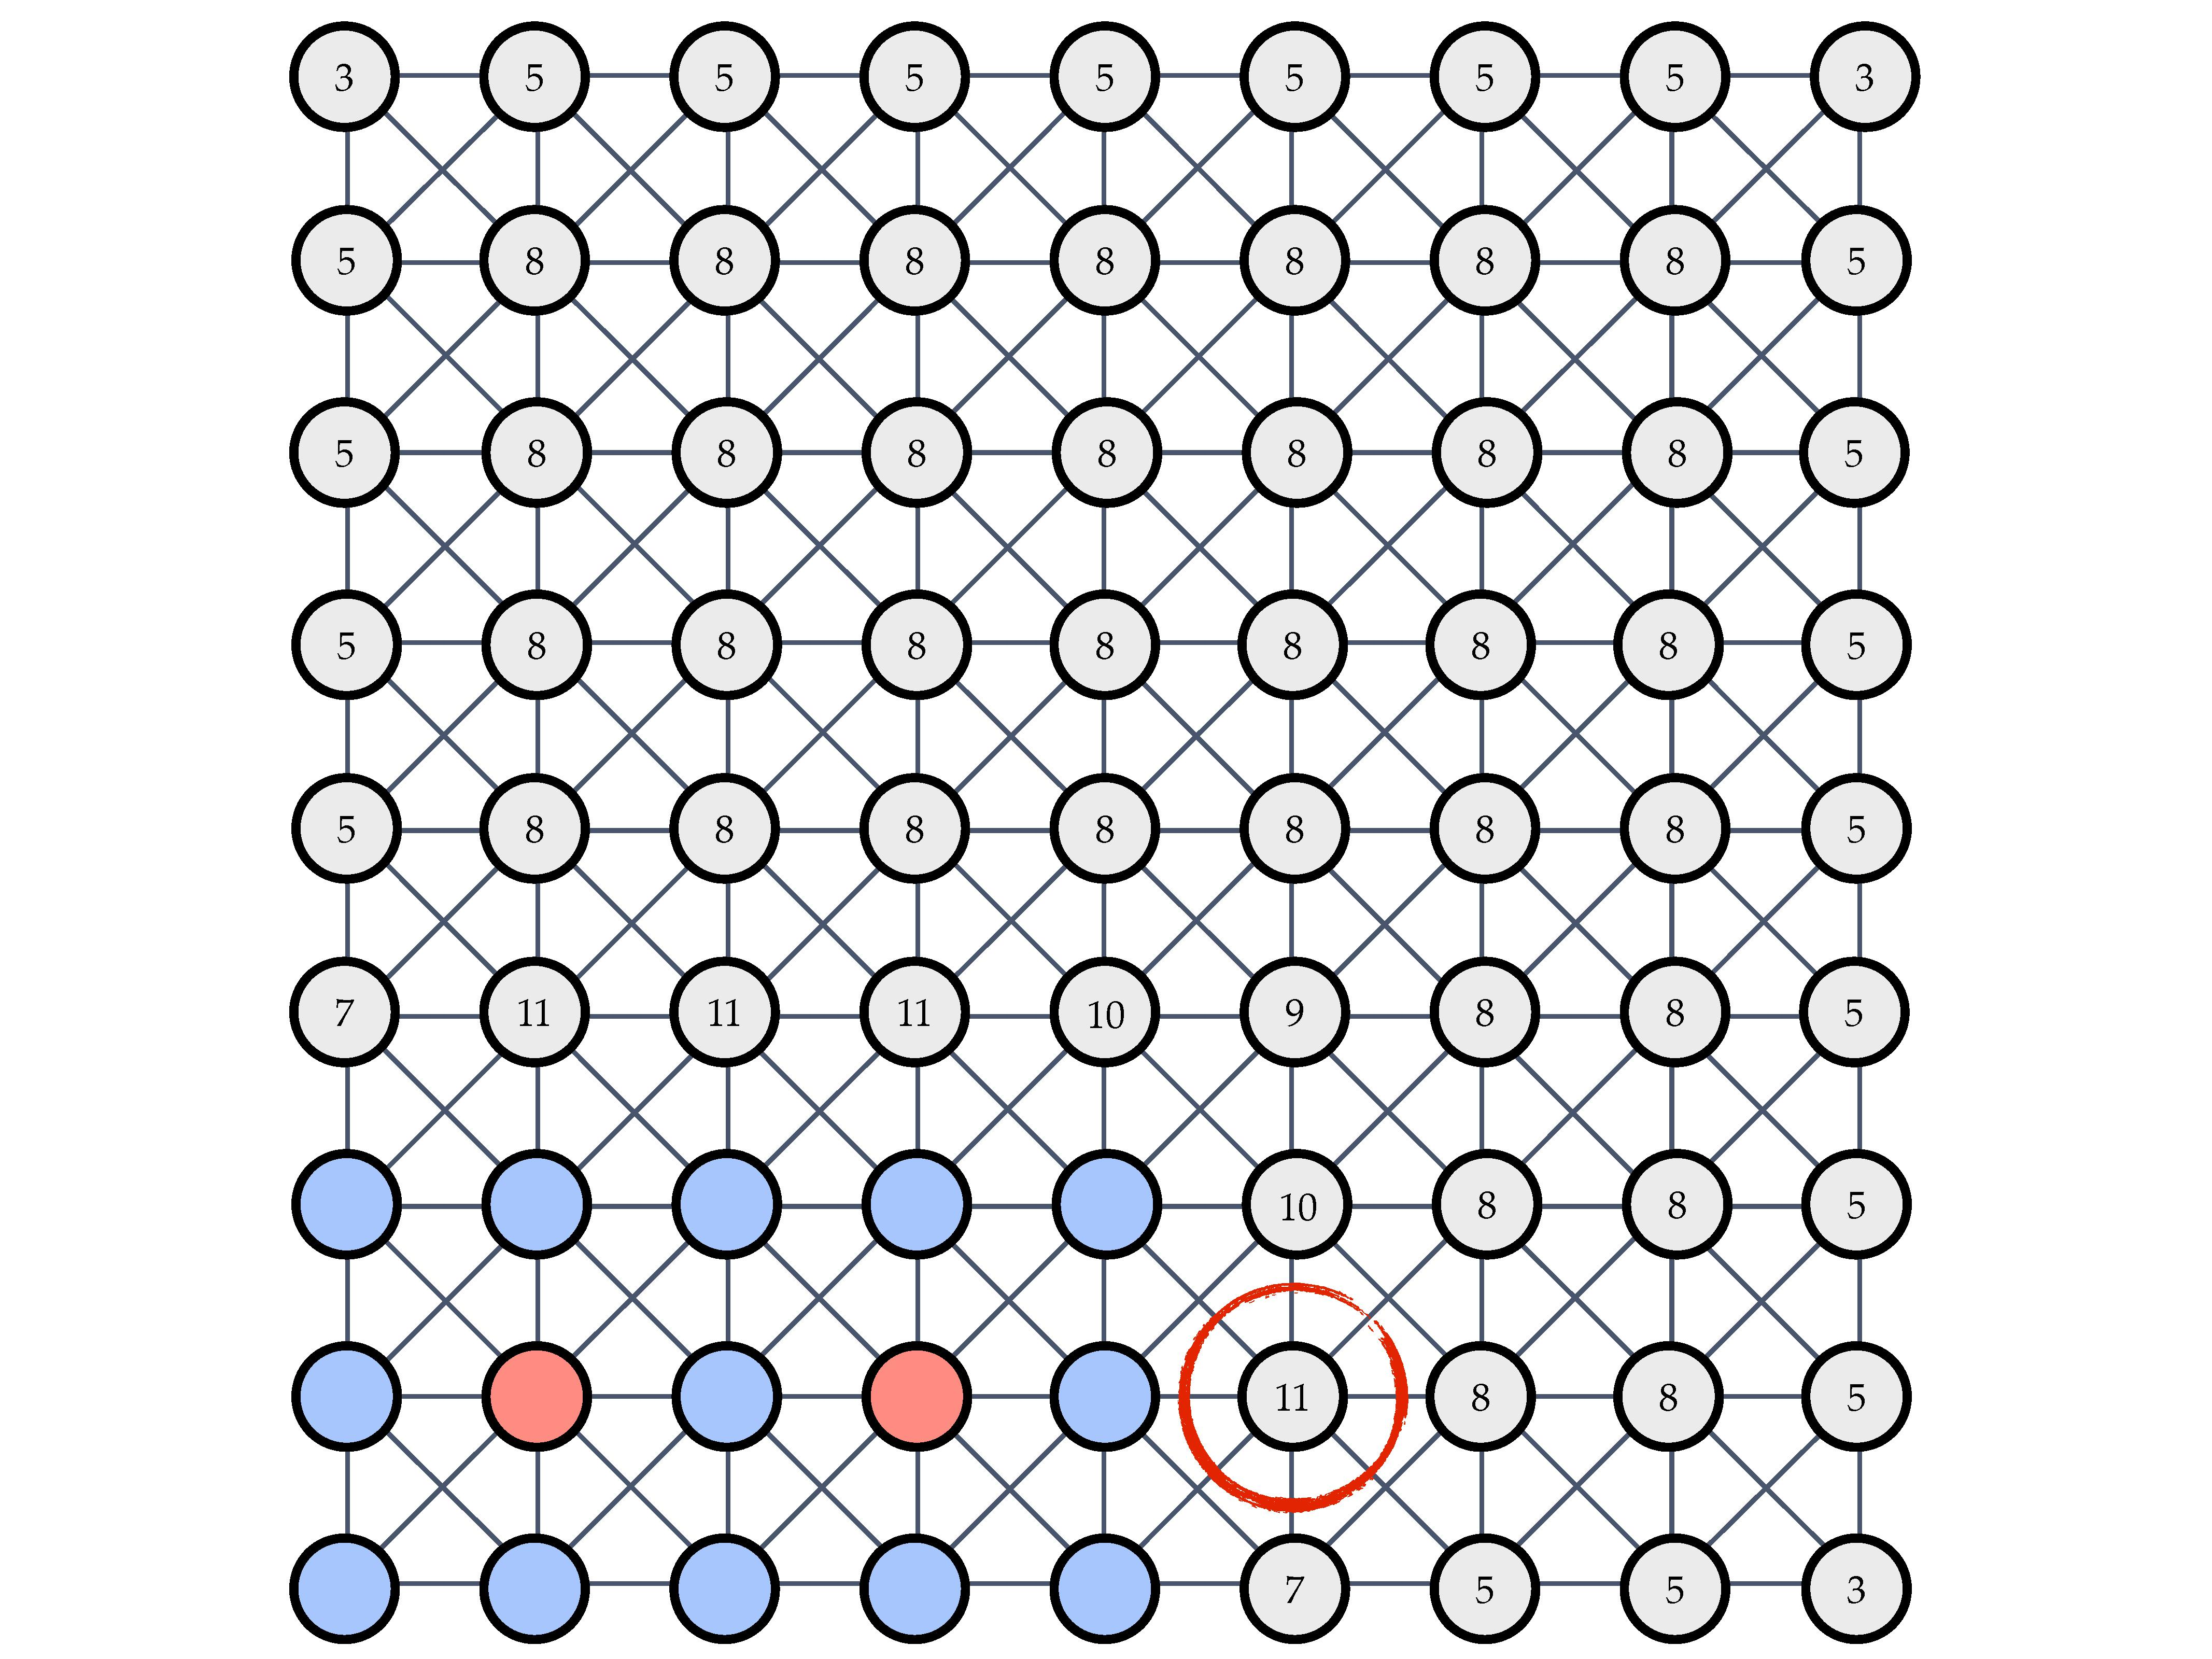
\includegraphics[width=0.7\textwidth]{../figures/amgCoarsening-6}
\end{center}}
\only<7>{
\begin{center}
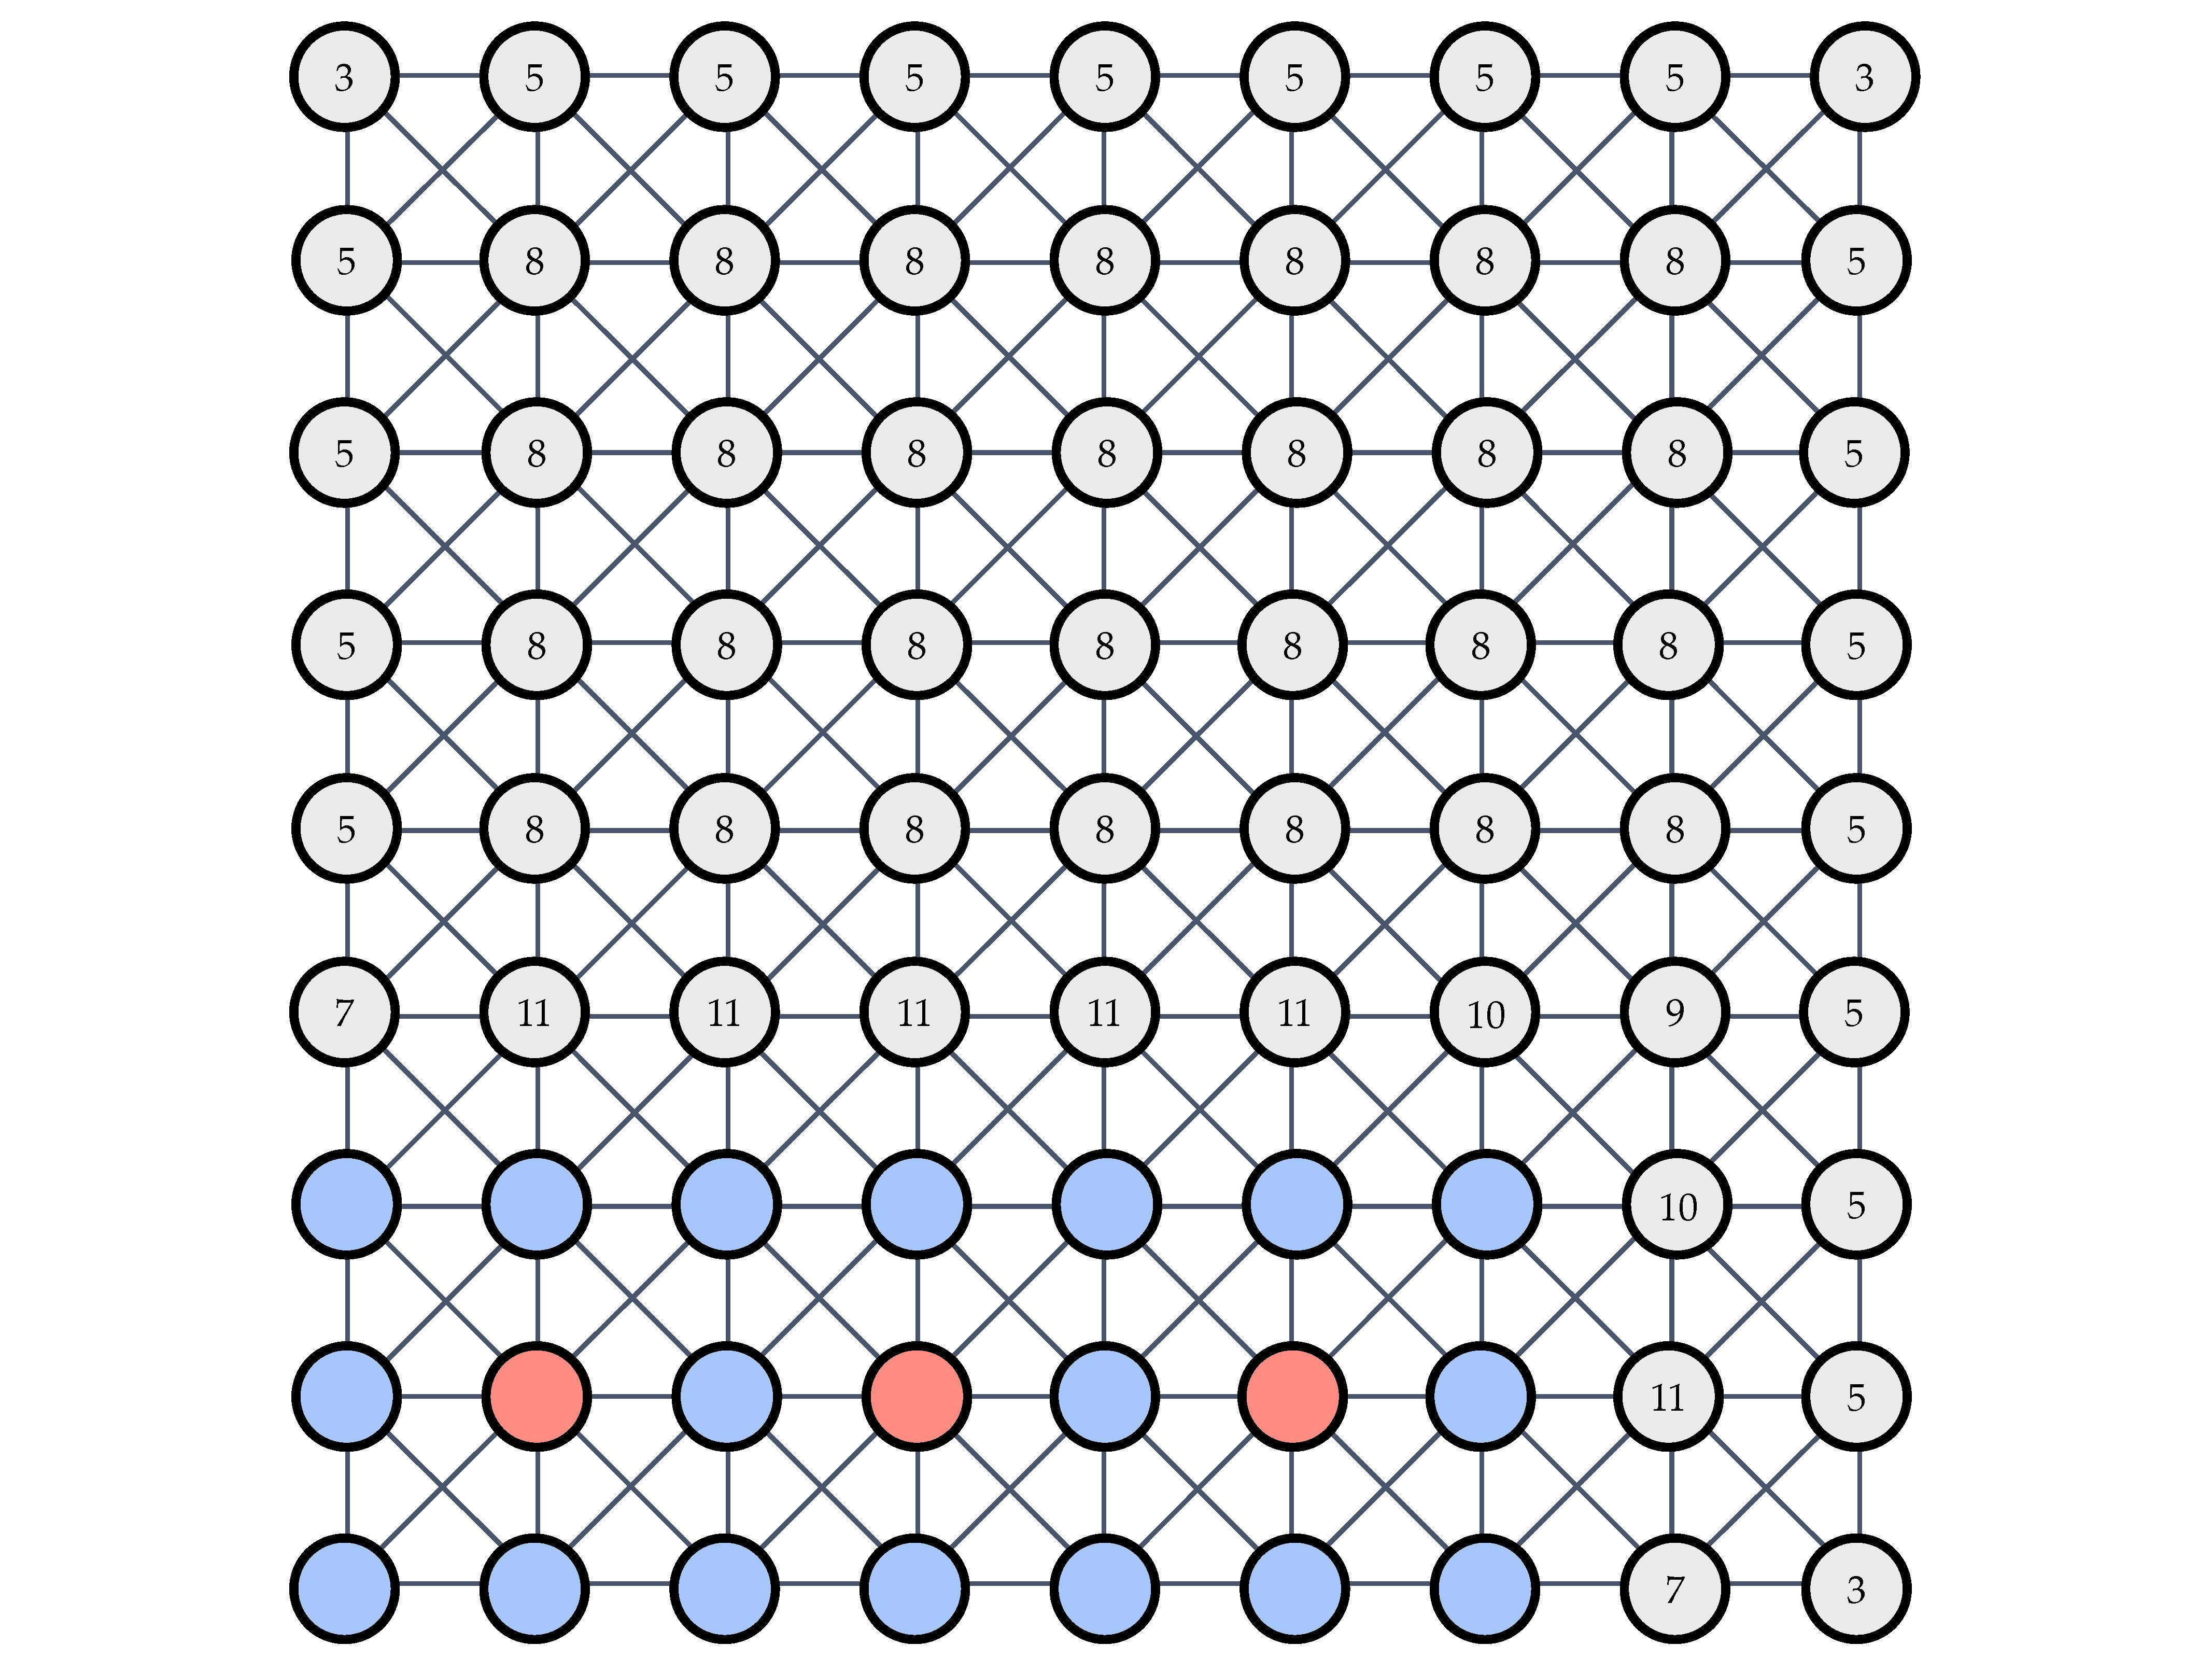
\includegraphics[width=0.7\textwidth]{../figures/amgCoarsening-7}
\end{center}}
\only<8>{
\begin{center}
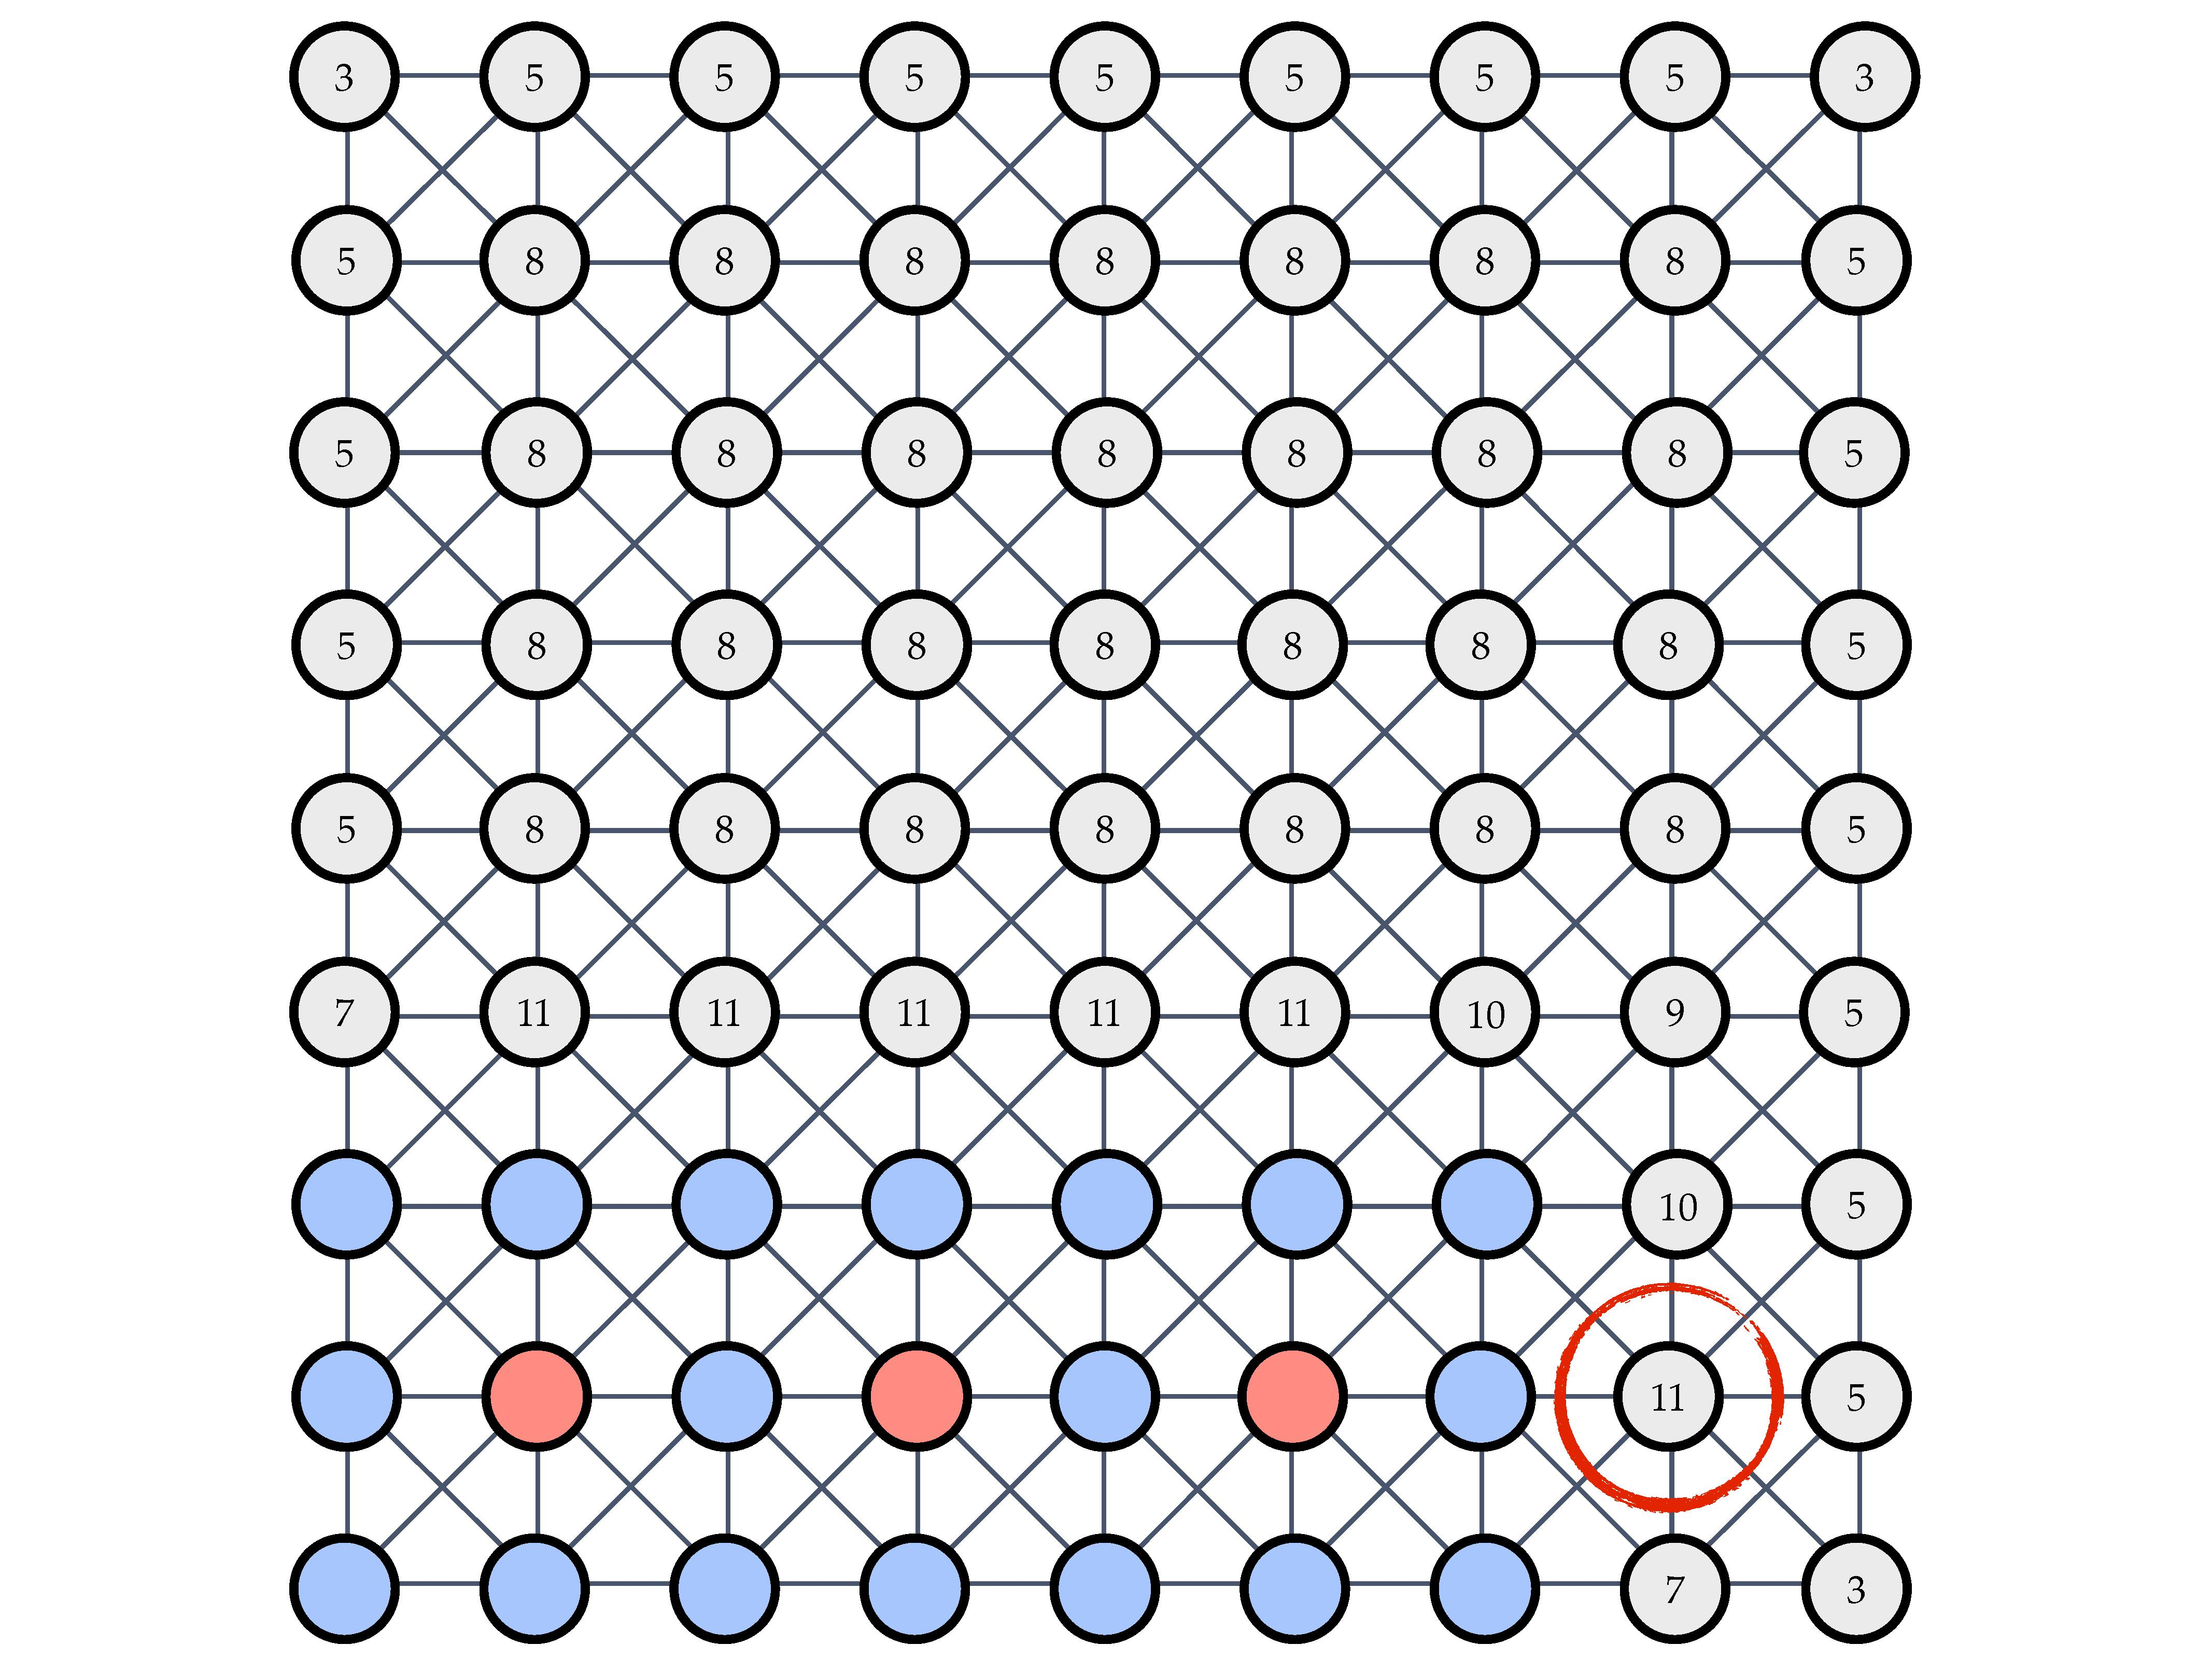
\includegraphics[width=0.7\textwidth]{../figures/amgCoarsening-8}
\end{center}}
\only<9>{
\begin{center}
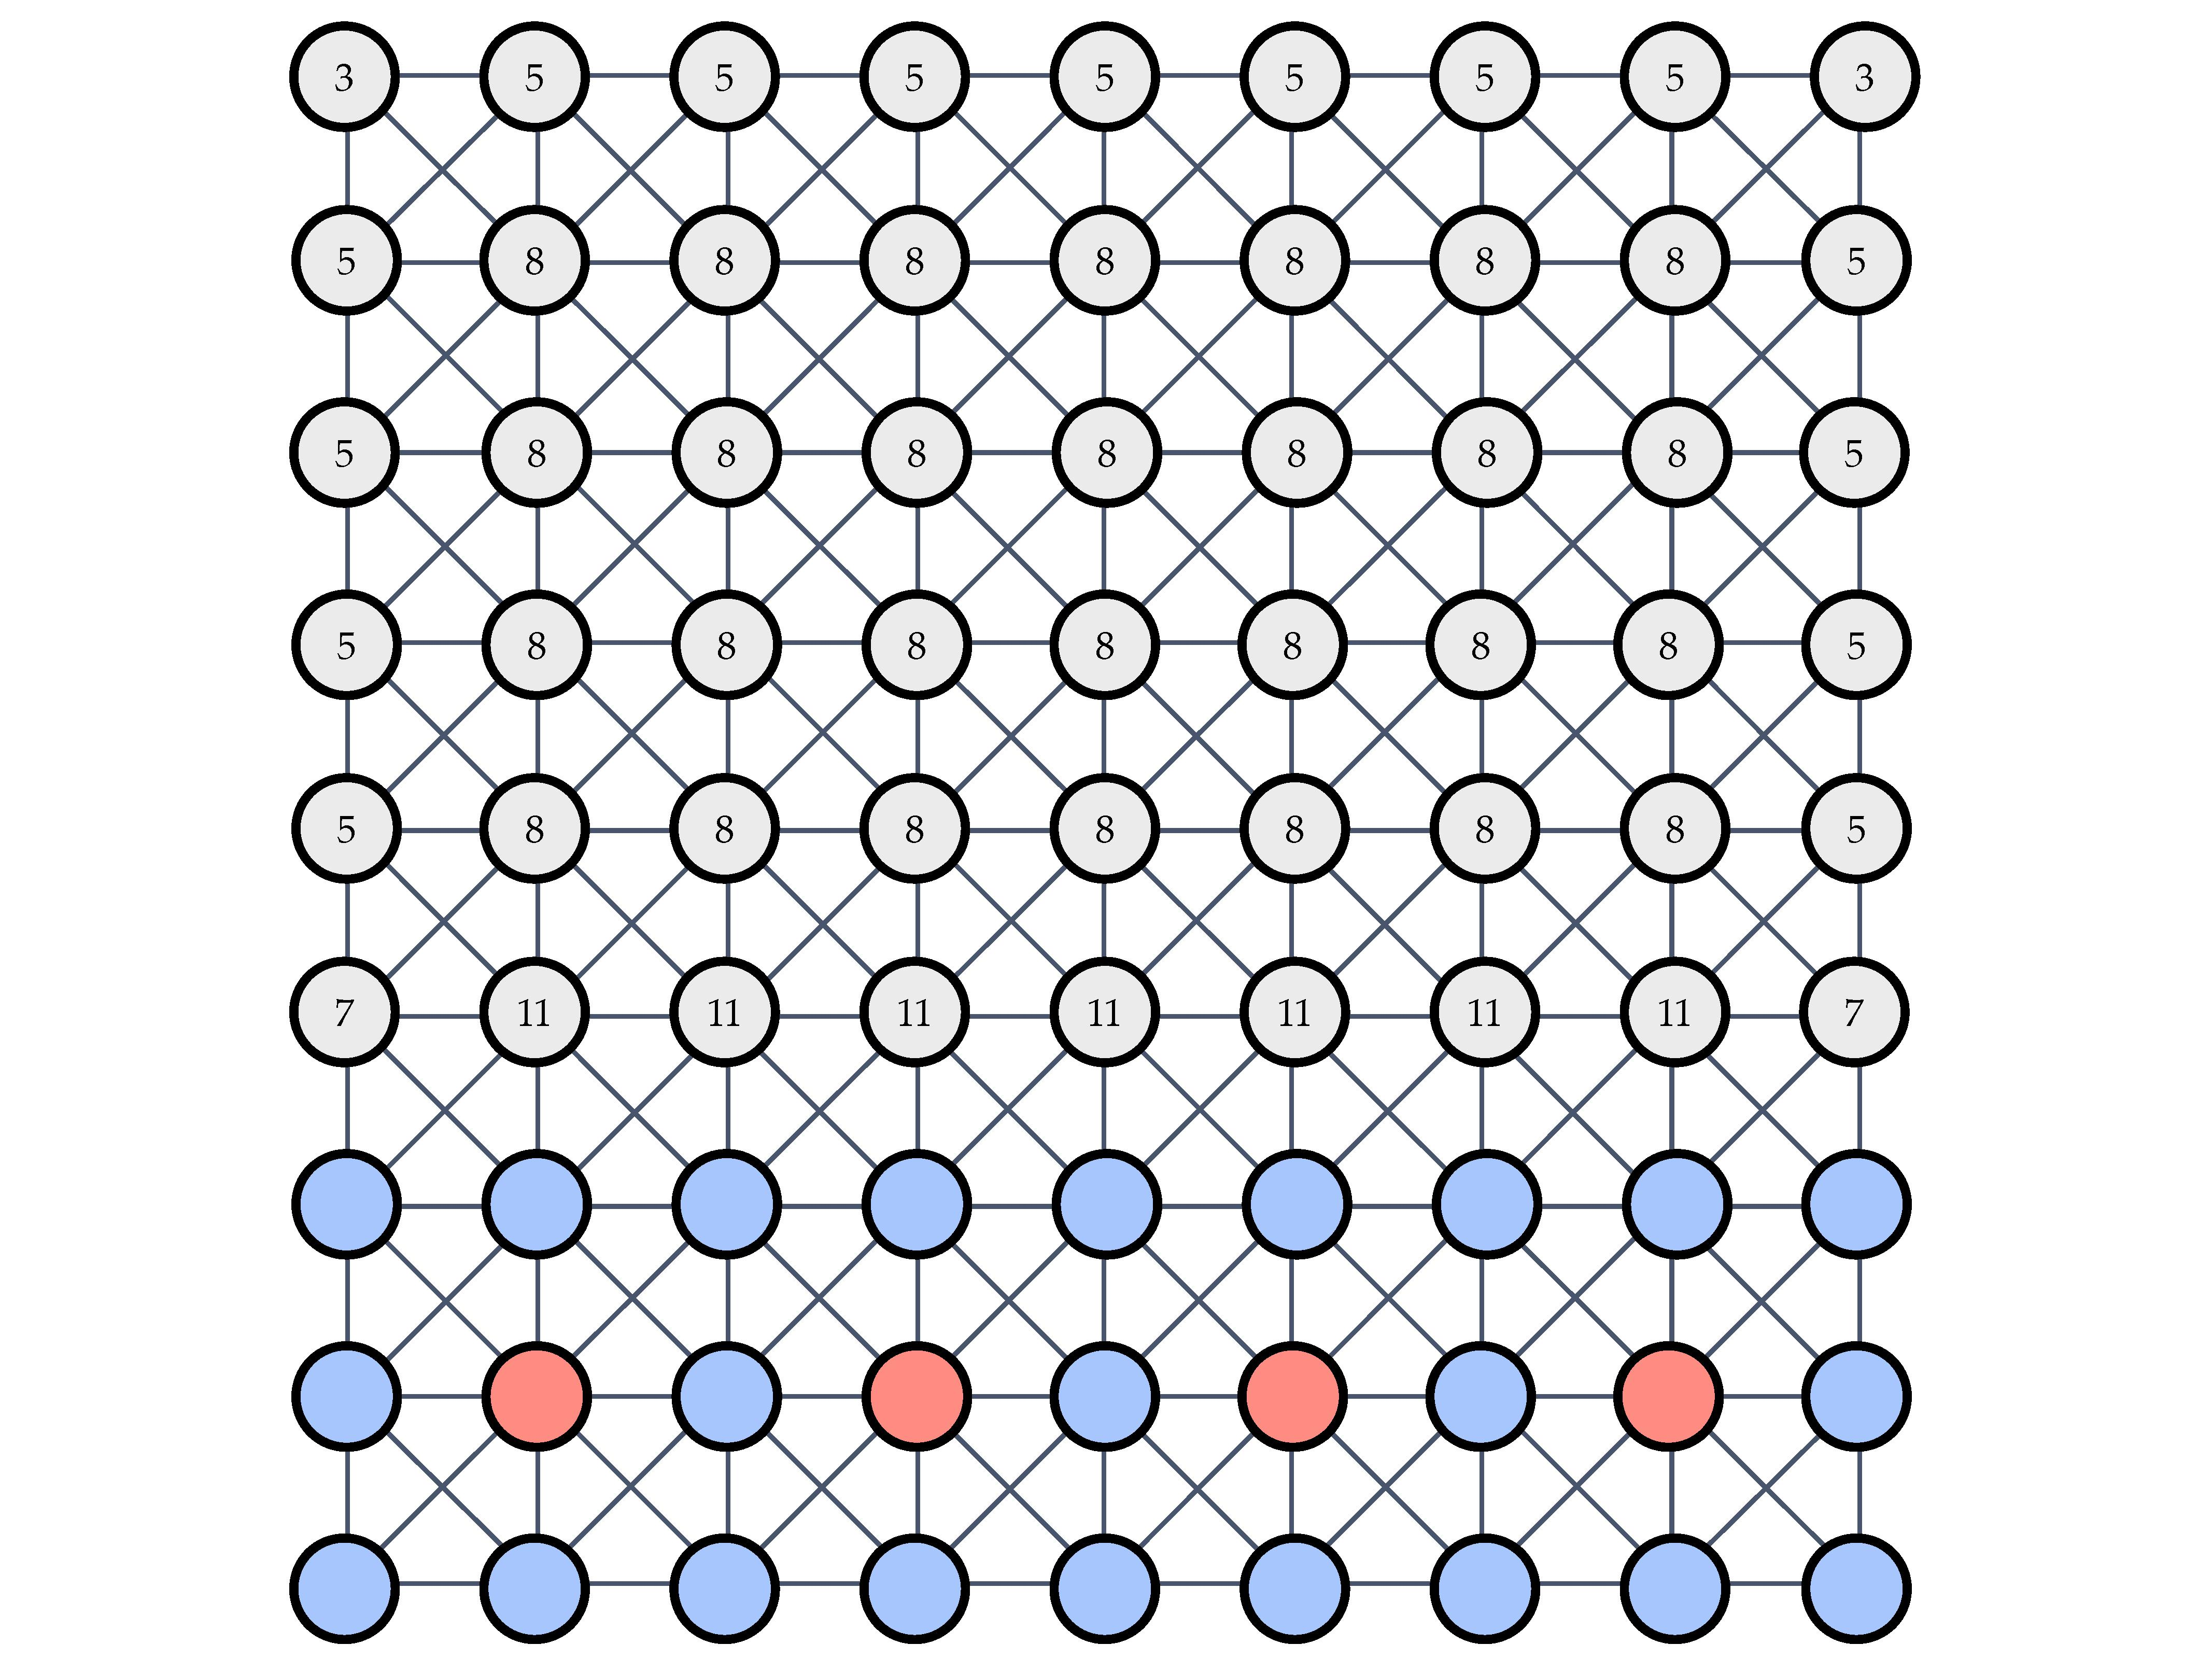
\includegraphics[width=0.7\textwidth]{../figures/amgCoarsening-9}
\end{center}}
\only<10>{
\begin{center}
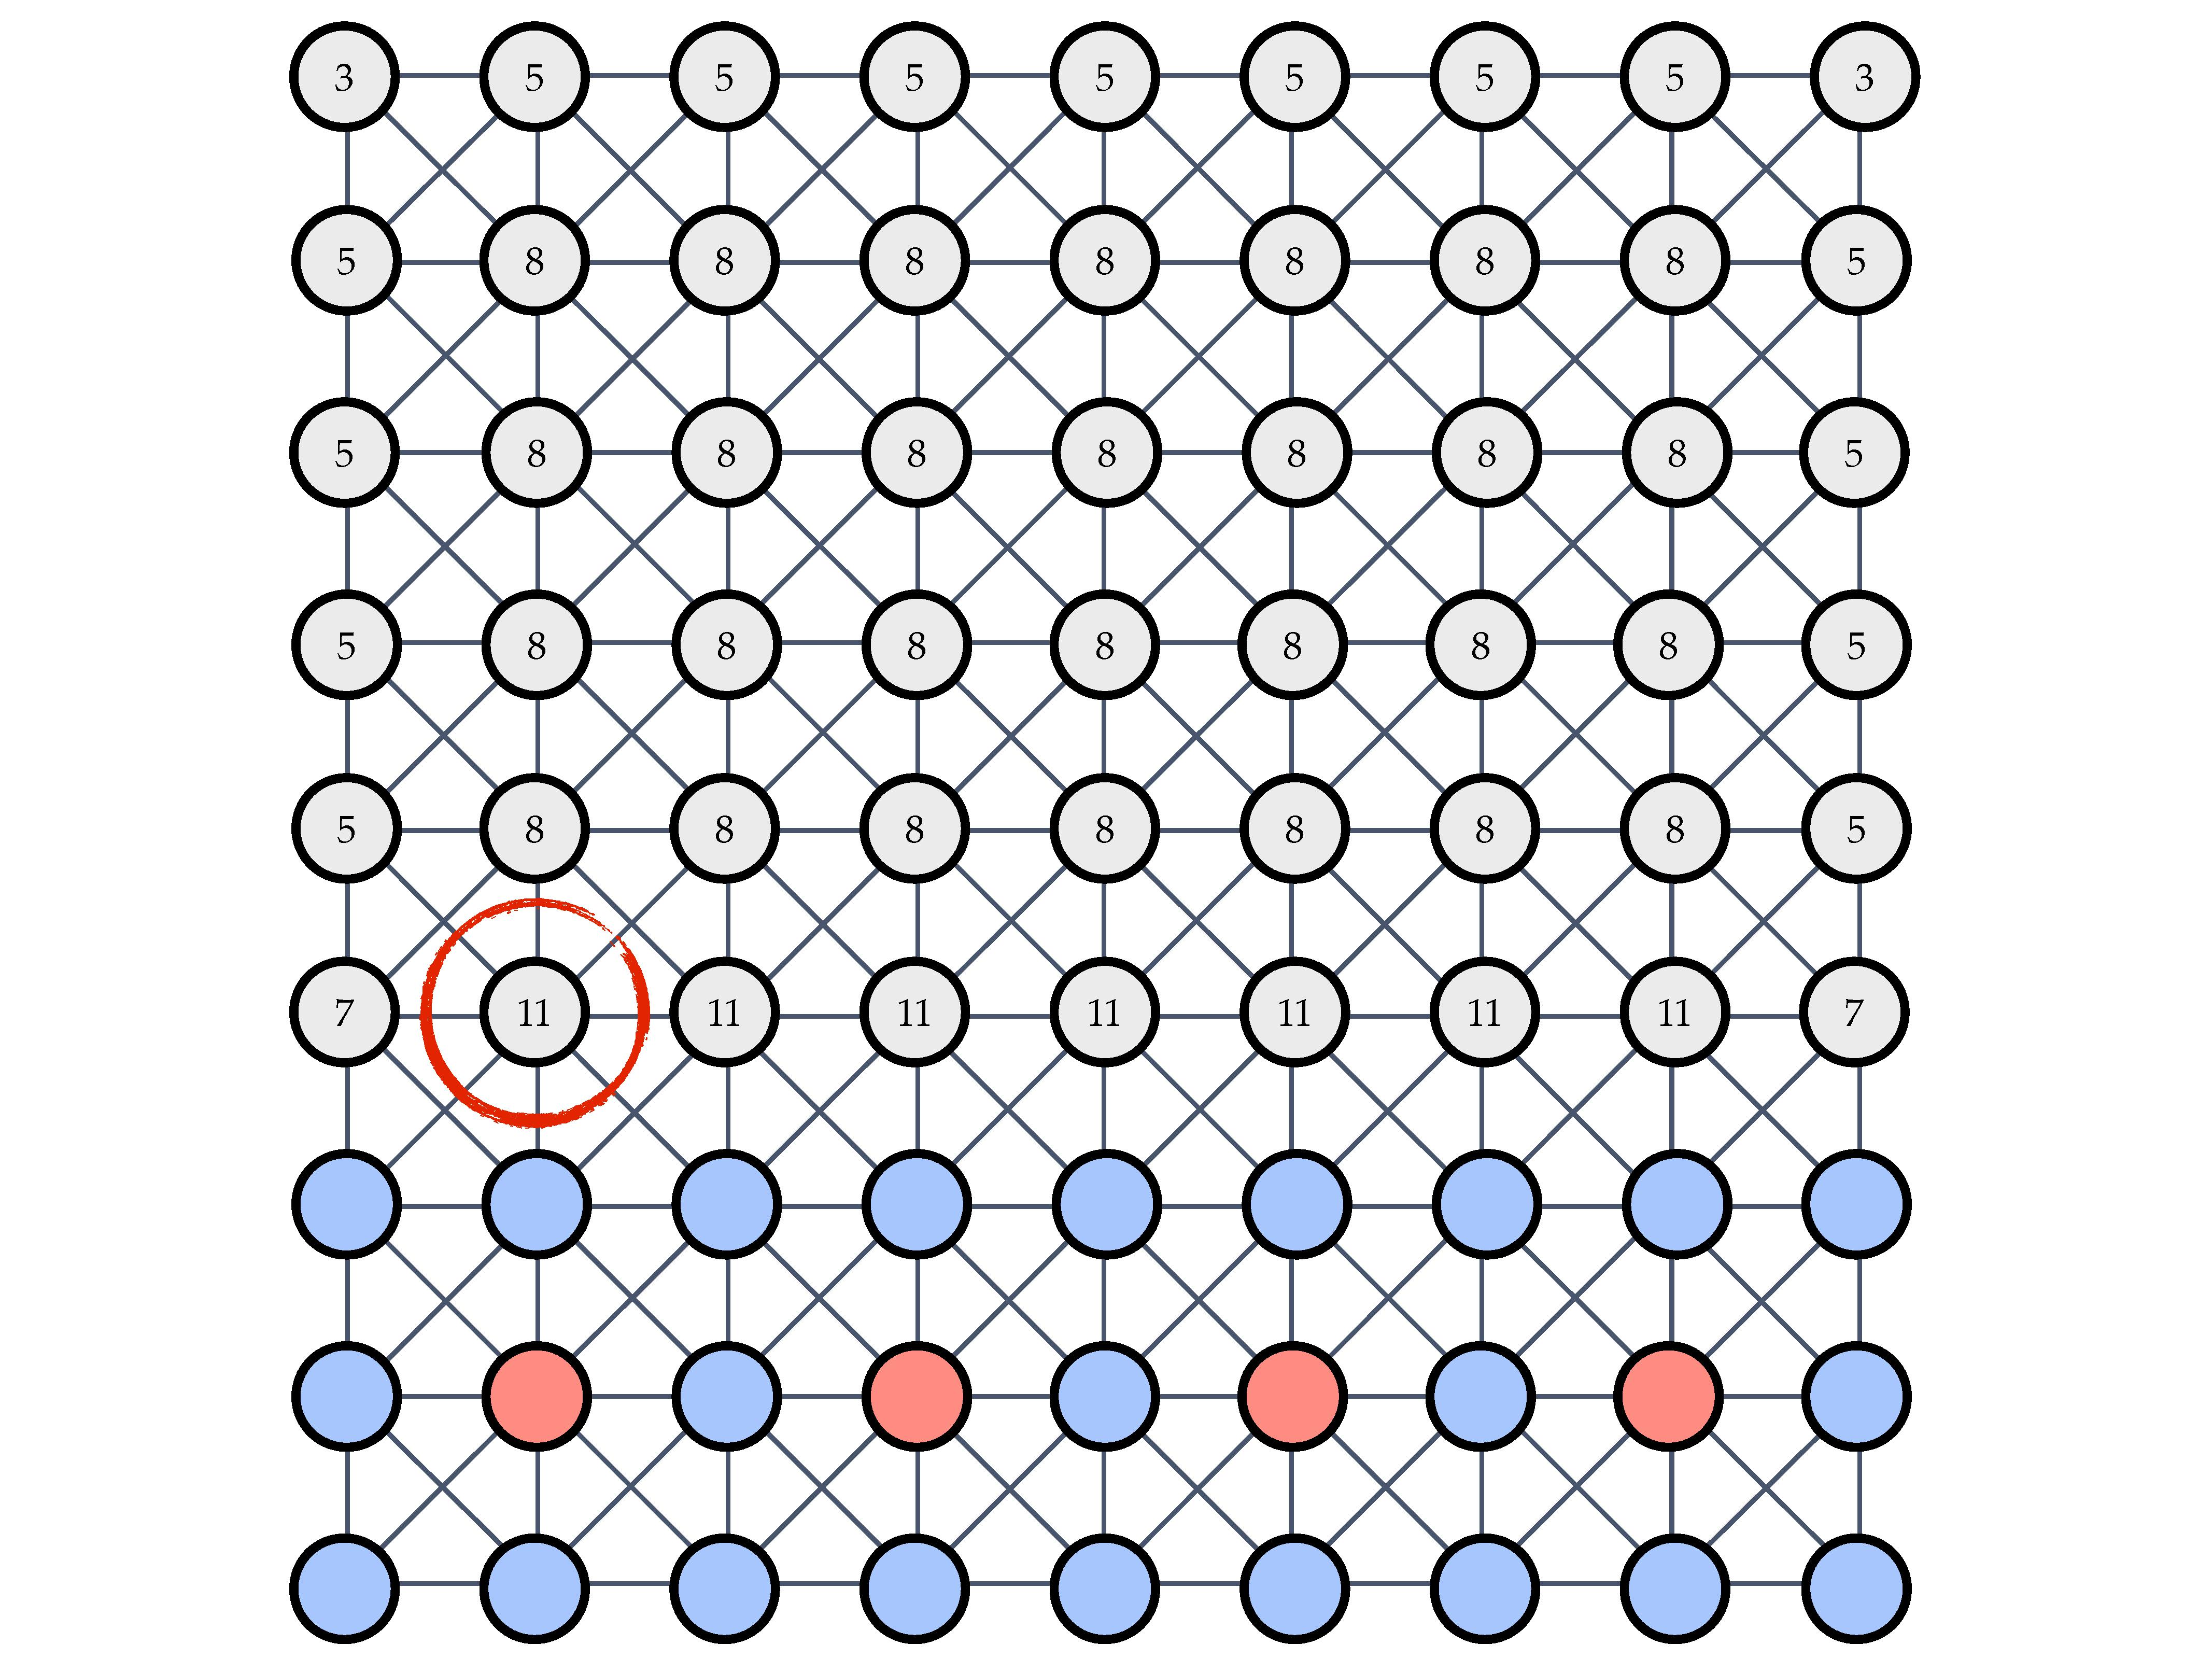
\includegraphics[width=0.7\textwidth]{../figures/amgCoarsening-10}
\end{center}}
\only<11>{
\begin{center}
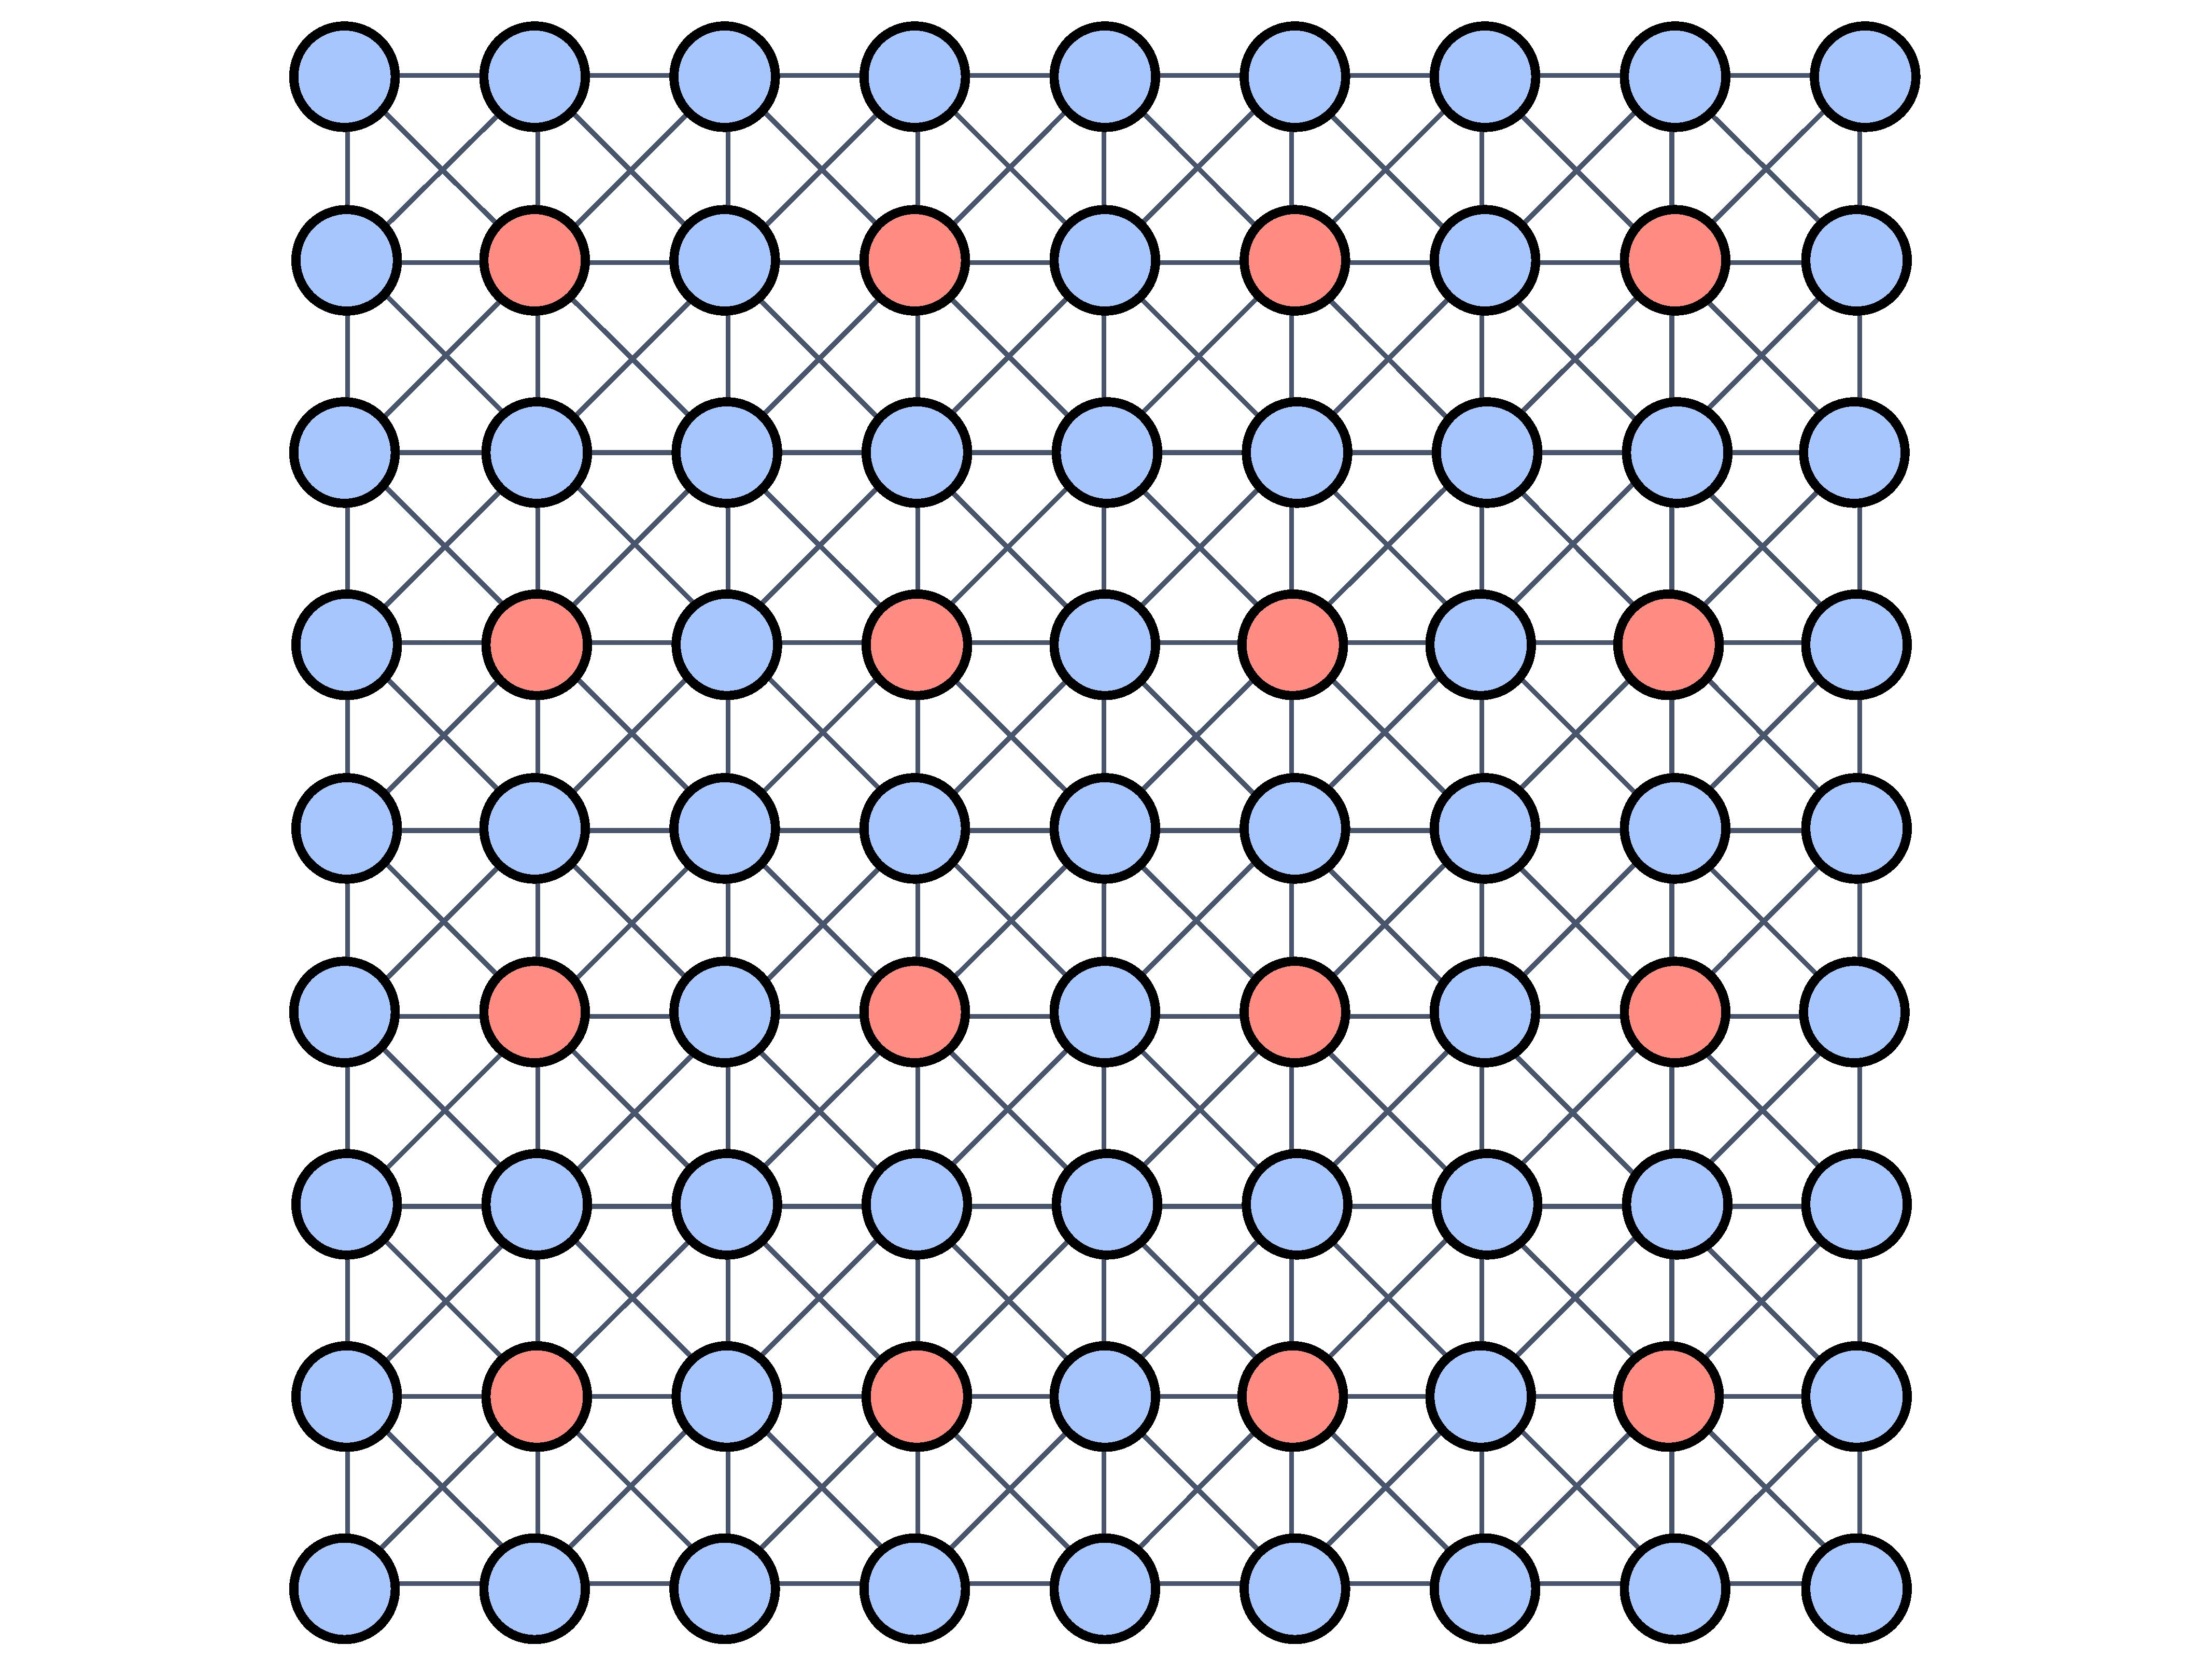
\includegraphics[width=0.7\textwidth]{../figures/amgCoarsening-11}
\end{center}}
\footnotesize{Slide credit: Luke Olson, Copper Mountain 2019 tutorial}
\end{frame}

% Slide
\begin{frame}{Coarsening}
\begin{block}{Coloring scheme}
\bit
\item The above example is done after one pass
\item Both heuristics are satisfied
\item Coarsening produced is the same as geometric coarsening
\eit
\end{block}
\end{frame}

% Slide
\begin{frame}{Coarsening}
\begin{block}{Coloring scheme}
\bit
\item Second pass switches some F-points to C-points to enforce heuristic 1
\item Not always used in practice
\eit
\end{block}
\end{frame}

% Slide
\begin{frame}{Coarsening}
\begin{block}{Benefits of the coloring scheme}
\bit
\item Completely algebraic method for coarsening
\item Incorporates strength of connection
\item Automatically generates appropriate coarsenings that must be hand-selcted in GMG, e.g. semi-coarsening for anisotropic problems
\eit
\end{block}
\end{frame}

% TODO (or in exercises) Show that you naturally get semicoarsening for grid-aligned anisotropy

%%%%%%%%%%%%%%%%%%%%%%%%%%%%%%%%%%%%%%%%%%%%%%%%%%%%%%%%%%%%%%%%%%%%%%%%%%%%%%%%

\section{Coarse grid operators}

% Slide
\begin{frame}{Coarse grid operators}
\begin{block}{Coarse grid operators}
\bit
\item Coarsening and interpolation are defined
\item Still need restriction and coarse-grid operators
\item Typical choice of restriction: $R = P^T$
\item Galerkin coarse-grid operator: $A^c = RAP = P^TAP$
\eit
\end{block}
\end{frame}

% Slide
\begin{frame}{Coarse grid operators}
\begin{block}{Optimality in $A$-norm}
\bit
\item Choosing $A^c = P^TAP$ provides optimal coarse-grid correction in the $A$-norm
\item Recall coarse-grid correction
\eit
\eq{
   \mathbf{u} \leftarrow \mathbf{u} + P(A^c)^{-1}R(\mathbf{f} - A\mathbf{u})
}
\end{block}
\end{frame}

% Slide
\begin{frame}{Coarse grid operators}
\begin{block}{Optimality in $A$-norm}
\bit
\item Error propagator for coarse-grid correction
\eq{
   \mathbf{e} &\leftarrow \mathbf{e} - P(A^c)^{-1}RA\mathbf{e} \\
   \mathbf{e} &\leftarrow (I - P(P^TAP)^{-1}P^TA)\mathbf{e}
}
\item So coarse-grid correction applies $(I - P(P^TAP)^{-1}P^TA)$ to the error
\item Want $(P(P^TAP)^{-1}P^TA)\mathbf{e}$ to be a good approximation to $\mathbf{e}$
\eit
\end{block}
\end{frame}

% Slide
\begin{frame}{Coarse grid operators}
\begin{block}{Optimality in $A$-norm}
\bit
\item Correction provided is in the range of interpolation, $Ran(P)$
\item The best correction in the $A$-norm is obtained by the minimization
\eq{
   \min_{\mathbf{v}\in Ran(P)} ||\mathbf{e} - \mathbf{v}||_A
}
\item The minimum is obtained by the orthogonal projection onto $Ran(P)$
\eit
\end{block}
\end{frame}

% Slide
\begin{frame}{Coarse grid operators}
\begin{block}{Optimality in $A$-norm}
\bit
\item Can check that $\pi = (P(P^TAP)^{-1}P^TA)$ is an $A$-orthogonal projection
\bit
\item \pi^2 = \pi
\itme \langle \pi \mathbf{x}, A \mathbf{y} \rangle = \langle \mathbf{x}, A \pi\mathbf{y} \rangle
\eit
\item Thus, the AMG coarse-grid correction is the best possible correction (in the $A$-norm) in the range of $P$
\eq{
   \min_{\mathbf{v}\in Ran(P)} ||\mathbf{e} - \mathbf{v}||_A = ||\mathbf{e} - (P(P^TAP)^{-1}P^TA)\mathbf{e}||_A
}
\eit
\end{block}
\end{frame}

% Slide
\begin{frame}{Coarse grid operators}
\begin{block}{Coase grid operator complexity}
\bit
\item Cost of GMG is straightforward to determine
\item Cost of AMG is less predictable
\item Coarse-grid operators tend to 
\eit
\end{block}
\end{frame}

% TODO Other things to finish up? Strengths or pitfalls to show?
% TODO Mention coarse grid complexity issues.

%%%%%%%%%%%%%%%%%%%%%%%%%%%%%%%%%%%%%%%%%%%%%%%%%%%%%%%%%%%%%%%%%%%%%%%%%%%%%%%%

\end{document}

